% !TEX encoding = UTF-8
% !TEX program = pdflatex
% !TEX spellcheck = en_GB

\documentclass[english,a4paper]{europasscv}

\ecvname{Todor Dimitrov Balabanov}
\ecvaddress{dist. "Mladost" 1, bl. 18, et. 5, fl. 6, app. 16, \\ 1750 Sofia, Bulgaria}
\ecvtelephone[+359 89 8237103]{+359 2 8764645}
\ecvemail{todor.balabanov@gmail.com}
\ecvhomepage{linkedin.com/in/todor-balabanov}
%\ecvim{AOL Messenger}{todor.balabanov}
\ecvim{Google Talk}{todor.balabanov}

\ecvdateofbirth{12 February 1980}
\ecvnationality{Bulgarian}
\ecvgender{Male}

\ecvpicture[width=3.8cm]{picture.png}

\begin{document}
  \begin{europasscv}

  \ecvpersonalinfo

  \ecvbigitem{Job applied for}{Research Team Member}

  \ecvsection{Work experience}
  
  \ecvtitle {September 2019 - present} {Software Developer}
  \ecvitem {} {Omega Systems Ltd., Sofia, Bulgaria}
  \ecvitem {} {Writing code and quality assurance in decision-making software projects.}
  \ecvitem {} {\ecvhighlight {Sector} \quad Software Production \& Support}
  
  \ecvtitle {October 2019 - So far} {Assistant Chief}
  \ecvitem {} {Institute of Information and Communication Technologies at the Bulgarian Academy of Sciences, Sofia, Bulgaria}
  \ecvitem {} {Participate in research projects, publish research findings, and teach. Main areas of research - modelling, optimization, decision support systems, Monte Carlo simulations, artificial neural networks, and evolutionary algorithms.}
  \ecvitem {} {\ecvhighlight {Sector} \quad Science \& Education}
  
  \ecvtitle {May 2012 - October 2019} {Software Developer}
  \ecvitem {} {Institute of Information and Communication Technologies at the Bulgarian Academy of Sciences, Sofia, Bulgaria}
  \ecvitem {} {Writing program code in research projects. Major areas of software implementation - modelling, optimization, decision support systems, Monte Carlo simulations, artificial neural networks and evolutionary algorithms.}
  \ecvitem {} {\ecvhighlight {Sector} \quad Science \& Education}
  
  \ecvtitle {September 2017 - September 2017} {Secondary School Teacher}
  \ecvitem {} {Private Profiled High School Educational Technology Ltd., Sofia, Bulgaria}
  \ecvitem {} {Preparation of study materials, conducting of training sessions, supervising the assimilation of the material by students in upper secondary school.}
  \ecvitem {} {\ecvhighlight {Sector} \quad Science \& Education}
  
  \ecvtitle {June 2012 - December 2012} {Software Developer}
  \ecvitem {} {Epic Dev Ltd., Sofia, Bulgaria}
  \ecvitem {} {Writing code and quality assurance in entertainment projects.}
  \ecvitem {} {\ecvhighlight {Sector} \quad Software Production and Support}
  
  \ecvtitle {February 2012 - April 2012} {Developer}
  \ecvitem {} {CBC Bulgaria EOOD, Sofia, Bulgaria}
  \ecvitem {} {Writing code and quality assurance in insurance software projects.}
  \ecvitem {} {\ecvhighlight {Sector} \quad Software Production and Support}
  
  \ecvtitle {August 2011 - January 2012} {Computer Application Developer}
  \ecvitem {} {FE-Design Bulgaria EOOD, Sofia, Bulgaria}
  \ecvitem {} {Writing code and quality assurance in software projects that implement the finite element method in materials testing.}
  \ecvitem {} {\ecvhighlight {Sector} \quad Software Production and Support}
  
  \ecvtitle {June 2010 - August 2011} {Database Developer}
  \ecvitem {} {Trade Unions, Sofia, Bulgaria}
  \ecvitem {} {Writing code, designing databases, and quality assurance in insurance software projects.}
  \ecvitem {} {\ecvhighlight {Sector} \quad Insurance \& Finance}
  
  \ecvtitle {July 2008 - November 2008} {Developer}
  \ecvitem {} {Interactive Engineering Ltd., Sofia, Bulgaria}
  \ecvitem {} {Writing code and quality assurance in entertainment projects.}
  \ecvitem {} {\ecvhighlight {Sector} \quad Software Production and Support}
  
  \ecvtitle {March 2008 - April 2008} {Developer}
  \ecvitem {} {Folio 3 Bulgaria EOOD, Sofia, Bulgaria}
  \ecvitem {} {Writing code and quality assurance in entertainment projects.}
  \ecvitem {} {\ecvhighlight {Sector} \quad Software Production \& Support}
  
  \ecvtitle {November 2007 - February 2008} {Developer}
  \ecvitem {} {About Sist Labs Ltd., Sofia, Bulgaria}
  \ecvitem {} {Writing program code and quality assurance in automotive embedded system projects.}
  \ecvitem {} {\ecvhighlight {Sector} \quad Software Production \& Support}
  
  \ecvtitle {January 2007 - September 2007} {Developer}
  \ecvitem {} {Casino Technology AD, Sofia, Bulgaria}
  \ecvitem {} {Writing code and quality assurance in gambling projects.}
  \ecvitem {} {\ecvhighlight {Sector} \quad Software Production \& Support}

  \ecvtitle {October 2006 - December 2006} {Developer}
  \ecvitem {} {Playtech Bulgaria EOOD, Sofia, Bulgaria}
  \ecvitem {} {Writing code and quality assurance in gambling projects.}
  \ecvitem {} {\ecvhighlight {Sector} \quad Software Production and Support}
  
  \ecvtitle {July 2006 - September 2006} {Data Transfer Machine Operator}
  \ecvitem {} {Hula \& Co., Human Dinex KG, Sofia, Bulgaria}
  \ecvitem {} {Processing information related to the selection of highly qualified staff in various areas of public administration.}
  \ecvitem {} {\ecvhighlight {Sector} \quad Recruitment}
  
  \ecvtitle {June 2006 - June 2006} {Developer}
  \ecvitem {} {Icom Ltd., Sofia, Bulgaria}
  \ecvitem {} {Writing code and quality assurance in embedded system and web application projects.}
  \ecvitem {} {\ecvhighlight {Sector} \quad Software Production \& Support}

  \ecvtitle {October 2005 - August 2006} {Computer Systems Software Application Specialist}
  \ecvitem {} {Institute of Information Technology at the Bulgarian Academy of Sciences, Sofia, Bulgaria}
  \ecvitem {} {Writing program code in research projects. Major Areas of Software Conversion - Pattern Recognition.}
  \ecvitem {} {\ecvhighlight {Sector} \quad Science \& Education}
  
  \ecvtitle {July 2003 - October 2003} {Secondary School Teacher}
  \ecvitem {} {68 Acad. Nikola Obreshkov High School, Sofia, Bulgaria}
  \ecvitem {} {Preparation of study materials, conducting of training sessions, controlling the absorption of the material by students in upper secondary school.}
  \ecvitem {} {\ecvhighlight {Sector} \quad Science \& Education}
  
  \ecvtitle {March 2003 - June 2003} {Computer Systems Software Specialist}
  \ecvitem {} {Multimedia Ltd., Sofia, Bulgaria}
  \ecvitem {} {Writing code and quality assurance in web application projects.}
  \ecvitem {} {\ecvhighlight {Sector} \quad Science \& Education}
  
  \ecvtitle {October 2000 - March 2001} {Electrical Engineer}
  \ecvitem {} {Medicom Ltd., Sofia, Bulgaria}
  \ecvitem {} {Repair and maintenance of X-ray machines.}
  \ecvitem {} {\ecvhighlight {Sector} \quad Health}
  
  \ecvsection{Education and training}
  
  \ecvtitlelevel{2009--2017}{PhD in Informatics and Computer Sciences}{}
  \ecvitem{}{Institute of Information and Communication Technologies at the Bulgarian Academy of Sciences, Sofia, Bulgaria}
  
  \ecvtitle{1998--2010}{Dip. Eng. BSc in Computer Systems and Technologies}
  \ecvitem{}{Technical University, Sofia, Bulgaria}
  
  \ecvtitle{2006--2008}{MSc in Internet Software Technologies}
  \ecvitem{}{New Bulgarian University, Sofia, Bulgaria}
  
  \ecvtitle{2002--2006}{BSc in Informatics}
  \ecvitem{}{New Bulgarian University, Sofia, Bulgaria}
  
  \ecvtitle{1993--1998}{Specialist in Programming Support Technology}
  \ecvitem{}{School of Technology Electronic Systems at the Technical University, Sofia, Bulgaria}
  
%   \pagebreak
  
  \ecvsection{Personal skills}

  \ecvmothertongue{Bulgarian}
  \ecvlanguageheader
  \ecvlanguage{English}{B1}{B2}{B2}{B2}{B2}
  \ecvlastlanguage{Russian}{A1}{A1}{A1}{A1}{A1}
  \ecvlanguagefooter
   
  \ecvblueitem{Communication skills}{ \begin{ecvitemize}
    \item Good communication skills in presentation to the audience, developed in many years of practice as a teacher.
    \item Good written communication skills, developed in the long-standing practice of writing popular and scientific articles.
    \item Experience in multicultural communication gained in work and life in the USA, Belgium and Estonia.
  \end{ecvitemize}}
  
  \ecvblueitem{Organisational / managerial skills}{\begin{ecvitemize}
    \item Vice-President of Smart Game Association, June 2016 - present
    \item Deputy Chairman of National Trade Union for Information and Communication Technologies - CITUB, May 2016 - present
    \item Owner and CEO of Velbazhd Software LLC, September 2008 - present
    \item Partner and CEO of Balgorit Ltd., August 2018 - May 2019
    \item Owner and CEO of ET TB Soft - Todor Balabanov, September 2008 - September 2010
    \item Erasmus for Young Entrepreneurs, July 2009 - September 2009
    \item CEED Bulgaria - Top Class - Entrepreneur, September 2008 - March 2009
  \end{ecvitemize}}
  
  \ecvblueitem{Computer skills}{ \begin{ecvitemize}
    \item Statistical data analysis
    \item Preprinting
    \item Programming
  \end{ecvitemize}}
  
  \ecvblueitem{Other skills}{\begin{ecvitemize}
     \item Mensa-Bulgaria SIGHT Program Coordinator from 2009 to 2016
     \item Operator of Radio Location Station at Bulgarian Army  - No20 / 536 - MoD. 46750 - 1996
  \end{ecvitemize}}

  \ecvblueitem{Driving licence}{B - active driver}
  
  \ecvsection{Additional information}

  \ecvblueitem{Teaching}{\begin{ecvitemize} \tiny
        \item BAS Training Center, Data Analysis with R-Lecturer, March 2019 - March 2019
    \item UniBIT-Sofia - Mobile Application Development - Lecturer, February 2019 - February 2019
    \item BAS Training Center, Data Analysis with R-Speaker, November 2018 - November 2018
    \item BAS Training Center, Data Analysis with R-Lecturer, April 2018 - April 2018
    \item Information Services AD - MS Excel - Advanced, MS Excel - Advanced - Database Analysis with PIVOT TABLE, MS Access - Lecturer, September 2018 - December 2018
    \item Information Services AD - MS Excel - Advanced, MS Excel - Advanced - Database Analysis with PIVOT TABLE, MS Access - Lecturer, September 2018 - December 2018
    \item Information Services AD - MS-Access - Lecturer, September 2018 - December 2018
    \item Information Services AD - MS-Access - Lecturer, 2018 - December 2018
    \item Information Services AD - Windows 7 (MS Word 2010, MS Excel 2010) - Lecturer, September 2018 - December 2018
    \item Information Services AD - Windows 7 (MS Word 2010, MS Excel 2010) - Lecturer, September 2018 - December 2018
    \item UniBIT-Sofia - Mobile Applications - Lecturer, January 2018 - May 2018
    \item BAS Training Center, Data Analysis with R-Lecturer, November 2017 - November 2017
    \item UniBIT-Sofia - Mobile Application Development - Lecturer, November 2017 - November 2017
    \item UniBIT-Sofia - Mobile Applications, February 2017 - May 2017
    \item UniBIT-Sofia - Mobile Application Development - Lecturer, December 2017 - December 2016
    \item UniBIT-Sofia - Introduction to Electronic Games Design, October 2016 - December 2016
    \item Soft Intellect Ltd. - Java Programming, April 2016 - July 2016
    \item Soft Intellect Ltd. - Introduction to Java, January 2016 - March 2016
    \item Information Services JSC - Databases - Lecturer, December 2014 - January 2015
    \item Information Services AD - Web Development (HTML, CSS, JavaScript) - Lecturer, November 2014 - December 2014
    \item Information Services AD - Introduction to C\# Programming - Lecturer, October 2014 - November 2014
    \item NBU-Sofia - Introduction to Java Programming - Lecturer, October 2014 - January 2015
    \item NBU-Sofia - Internet Programming - Lecturer, October 2014 - January 2015
        \item UniBIT-Sofia - Java Programming - Assistant, October 2014 - December 2014
    \item UniBIT-Sofia - Introduction to Programming - Assistant, October 2014 - December 2014
    \item NBU-Sofia - Current Trends in Internet Technologies - Lecturer, February 2014 - June 2014
    \item NBU-Sofia - Java for Advanced Lecturer, February 2014 - June 2014
    \item Information Services AD - Databases - Lecturer, March 2014 - July 2014
    \item UniBIT-Sofia - Programming Environments - Lecturer, February 2014 - May 2014
    \item UniBIT-Sofia - Wireless and Mobile Computing - Lecturer, February 2014 - May 2014
    \item IUC-Sofia - Information systems project management - lecturer, October 2013 - February 2014
    \item IUC-Sofia - Information system in business - lecturer, October 2013 - February 2014
    \item NBU-Sofia - Introduction to Java Programming - Lecturer, October 2013 - January 2014
    \item NBU-Sofia - Internet Programming - Lecturer, October 2013 - January 2014
    \item UniBIT-Sofia - Java Programming - Assistant, October 2013 - December 2013
    \item UniBIT-Sofia - Introduction to Programming - Assistant, October 2013 - December 2013
    \item Information Services AD - Java Programming for Advanced - Lecturer, March 2013 - July 2013
    \item NBU-Sofia - Java for Advanced Lecturer, February 2013 - June 2013
    \item IUC-Sofia - System analysis, development \& design - lecturer, February 2013 - May 2013
    \item IUC-Sofia - Information system legislation - Lecturer, February 2013 - May 2013
    \item IUC-Sofia - E-business management - lecturer, February 2013 - May 2013
    \item IUC-Sofia - Introduction to Databases / Database Applications - Lecturer, December 2012 - February 2013
    \item IUC-Sofia - Intro to Multimedia and the Internet - lecturer, December 2012 - February 2013
        \item NBU-Sofia - Introduction to Java Programming - Lecturer, October 2012 - January 2013
    \item Information Services AD - Introduction to Java Programming - Lecturer, September 2012 - October 2012
    \item NBU-Sofia - Java for Advanced Lecturer, February 2012 - June 2012
    \item NBU-Sofia - Introduction to Java Programming - Lecturer, October 2011 - January 2012
    \item Asgore Ltd. - C Programming for Beginners - Lecturer, June 2011 - July 2011
    \item NBU-Sofia - Java for Advanced Lecturer, February 2011 - June 2011
    \item TUES-Sofia - Programming - Practice of Lecturer, February 2011 - June 2011
    \item St. Ariadne College - Communication Technology - Lecturer, March 2011 - June 2011
    \item St. Ariadne College - Internet and Web Design Programming - Lecturer, March 2011 - June 2011
    \item NBU-Sofia - Introduction to Java Programming - Lecturer, October 2010 - January 2011
    \item TUES-Sofia - C Programming, September 2010 - January 2011
    \item NBU-Sofia - Java for Advanced Lecturer, February 2010 - June 2010
    \item TUES-Sofia - Programming - Practice of C-Lecturer, February 2010 - June 2010
    \item TUES-Sofia - Programming for the iPhone - lecturer, February 2010 - June 2010
    \item NBU-Sofia - Introduction to Java Programming - Lecturer, October 2009 - January 2010
    \item TUES-Sofia - Development of Open Source Projects by the Methodology Extreme Programming - Lecturer, October 2009 - January 2010
    \item TUES-Sofia - Web Development with PHP and MySQL - Lecturer, October 2009 - January 2010
    \item TUES-Sofia - C-speaker Programming, October 2009 - January 2010
    \item SPGE-Sofia - Java for Beginners - Lecturer, February 2009 - June 2009
    \item TUEEC-Sofia - Development of Open Source Projects by the Methodology Extreme Programming - Lecturer, February 2009 - June 2009
    \item Sofia University - Programming, Data Structures, Files and Objects Part I - Assistant, February 2009 - June 2009
    \item Sofia University - E-Business Systems Assistant, February 2009 - June 2009
    \item NBU-Sofia - Java for Advanced Lecturer, February 2009 - June 2009
    \item TU-Sofia - Programming Languages - Assistant, October 2008 - January 2009
    \item TU-Sofia - Computer Programming and Use 3 - Assistant, October 2008 - January 2009 
  \end{ecvitemize}}
  
  \ecvblueitem{Publications}{\begin{ecvitemize} \tiny
    \item \textit{Multilayer Perceptron Training Randomized by Second Instance of Multilayer Perceptron}, T Balabanov, I Zankinski, K Kolev, 13th Annual Meeting of the Bulgarian Section of SIAM, (2018).
    \item \textit{Weights Permutation in Multilayer Perceptron}, T Balabanov, I Zankinski, R Ketipov, International Conference on Big Data, Knowledge and Control Systems Engineering, (2018).
    \item \textit{Activation Function Permutation for Multilayer Perceptron Training}, T Balabanov, T Atanasova, I Blagoev, International Conference on Big Data, Knowledge and Control Systems Engineering, (2018).
    \item \textit{MLP with Stochastic Manipulated Hidden Layer}, T Balabanov, R Ketipov, Z Atanassova, International Scientific Conference UNITECH 2018, Gabrovo, Bulgaria, (2018).
    \item \textit{Greedy Genetic Algorithm Hybrid Solution of 1D Stock Cutting Problem}, T Balabanov, I Blagoev, Z Atanassova, International Scientific Conference UNITECH 2018, Gabrovo, Bulgaria, (2018).
    \item \textit{Self Rising Tri Layers MLP for Time Series Forecasting}, TD Balabanov, II Blagoev, KI Dineva, International Conference on Distributed Computer and Communication Networks, (2018).
    \item \textit{Optimization of String Rewriting Operations for 3D Fractal Generation with Genetic Algorithms}, T Balabanov, J Sevova, K Kolev, International Conference on Numerical Methods and Applications, (2018).
    \item \textit{Scientific calculations with Java and Android. Practical Guide}, T Balabanov, I Zankinski, P Tomov, Lectures on Computer Science and Technology at IICT-BAS, (2018).
    \item \textit{Distributed System for Time Series Forecasting with Evolutionary Algorithms and Artificial Neural Networks}, T Balabanov, Institute of Information and Communication Technologies, Bulgarian Academy of Sciences, (2017).
    \item \textit{Geometric Visualization of a Polygon Area Partitioning}, T Balabanov, S Darachev, I Jordanov, A Karakushev, N Kitanov, A Manov, G Nikolov, S Nonev, Z Nedyalkova, E Rogachev, N Stojkovikj, P Tomov, I Zankinsk, 12th Annual Meeting of the Bulgarian Section of SIAM, (2017).
    \item \textit{Slot Machine Reels Reconstruction with Genetic Algorithms}, P Tomov, I Zankinski, T Balabanov, 12th Annual Meeting of the Bulgarian Section of SIAM, (2017).
    \item \textit{Sound Vectorization with Genetic Algorithms}, P Tomov, I Zankinski, T Balabanov, 12th Annual Meeting of the Bulgarian Section of SIAM, (2017).
    \item \textit{Long Short Term Memory in MLP Pair}, T Balabanov, International Scientific Conference UniTech, (2017).
    \item \textit{Slot Machine Reels Reconstruction with Monte-Carlo Search}, P Tomov, I Zankinski, T Balabanov, International Scientific Conference UniTech, (2017).
    \item \textit{Alternative Activation Function Derivative in Artificial Neural Networks}, I Zankinski, P Tomov, T Balabanov, 25th Symposium with International Participation - Control of Energy, Industrial and Ecological Systems, Bankia, Bulgaria, (2017).
    \item \textit{Self-Organized Networks}, A Stojanova, D Bikov, G Kobeaga, M Kocaleva, T Koca, T Ashley, T Balabanov, Proceedings of the 131st European study group with industry, (2017).
    \item \textit{Authenticity management algorithm for digital images}, T Balabanov, N Manev, W Mudzimbabwe, P Tomov, I Zankinski, S Zheezova, 11th Annual Meeting of the Bulgarian Section of BGSIAM, (2016).
    \item \textit{Image construction with 2D ellipses by genetic algorithms optimization}, T Balabanov, M Barova, D Keremedchiev, 11th Annual Meeting of the Bulgarian Section of BGSIAM, (2016).
    \item \textit{Android Programming Practical Guide}, T Balabanov, IICT - BAS Lectures in Computer Science and Technology, (2016).
    \item \textit{Distributed System for Artificial Neural Networks Training Based on Mobile Devices}, T Balabanov, K Genova, International Conference AUTOMATICS AND INFORMATICS, (2016).
    \item \textit{Web Distributed Computing For Evolutionary Training Of Artificial Neural Networks}, T Balabanov, D Keremedchiev, I Goranov, International Conference InfoTech, (2016).
    \item \textit{AJAX Distributed System for Evolutionary Algorithms based Artificial Neural Networks Training}, T Balabanov, K Genova, Proceedings of the XXIV International Symposium Thermal Energy Management and Systems Management, Energy, Industrial and Environmental Management, (2016).
    \item \textit{Two Dimensional Optimal Cutting Problem}, A Avdzhieva, T Balabanov, G Evtimov, I Jordanov, N Kitanov, N Zlateva, (2016).
    \item \textit{Strategy for Individuals Distribution by Incident Nodes Participation in Star Topology of Distributed Evolutionary Algorithms}, T Balabanov, I Zankinski, M Barova, Cybernetics and Information Technologies, (2016).
    \item \textit{Distributed evolutional model for music composition by human-computer interaction}, T Balabanov, Proceedings of International Scientific Conference UniTech 2015 Gabrovo, (2015).
    \item \textit{Distributed evolutionary computing migration strategy by incident node participation}, T Balabanov, I Zankinski, M Barova, International Conference on Large-Scale Scientific Computing, (2015).
    \item \textit{Slot machine RTP optimization and symbols wins equalization with discrete differential evolution}, T Balabanov, I Zankinski, B Shumanov, International Conference on Large-Scale Scientific Computing, (2015).
    \item \textit{Statistical Models Optimization based on Differential Evolution and Monte-Carlo Evaluated Cost Function}, T Balabanov, I Zankinski, B Shumanov, Proceedings of the XXIII International Symposium Management of Energy, Industrial and Environmental Systems, (2015).
    \item \textit{Optimal Cutting Problem}, A Avdzhieva, T Balabanov, G Evtimov, D Kirova, H Kostadinov, T Tsachev, S Zhelezova, N Zlateva, FASTUMPRINT, Sofia, Bulgaria, (2015).
    \item \textit{Avoiding Local Optimums in Distributed Population based Heuristic Algorithms}, T Balabanov, Proceedings of the XXIII International Symposium Management of Energy, Industrial and Environmental Systems, (2015).
    \item \textit{Slot machines RTP optimization with genetic algorithms}, T Balabanov, I Zankinski, B Shumanov, International Conference on Numerical Methods and Applications, (2014).
    \item \textit{The Eclipse Multilanguage Integrated Application Development Environment}, A Chikalanov, T Balabanov, Behind the letters - About the Writer, (2014).
    \item \textit {Population Algorithms for the Training of Artificial Neural Networks in Outdoor Games}, T Balabanov, Proceedings of the First National Thematic School and the Exchange for Scientific Ideas in Information and Communication Technologies, (2013).
    \item \textit{Time Series Prediction by Artificial Neural Networks and Differential Evolution in Distributed Environment}, T Balabanov, I Zankinski, N Dobrinkova, International Conference on Large-Scale Scientific Computing, (2011).
    \item \textit{Heuristic Forecasting Approaches in Distributed Environment}, T Balabanov, Proceedings of Anniversary Scientific Conference 40 Years Department of Industrial Automation, (2011).
    \item \textit{Predicting time series with artificial neural networks and differential evolution in a distributed environment}, T Balabanov, I Zankinsky, V Simeonova, IIT Working Papers, IIT / WP-268B, (2010).
    \item \textit{Library for image co-registration with application for mosaicing}, T Balabanov, New Bulgarian University, (2006).
  \end{ecvitemize}}
  
  \end{europasscv}

%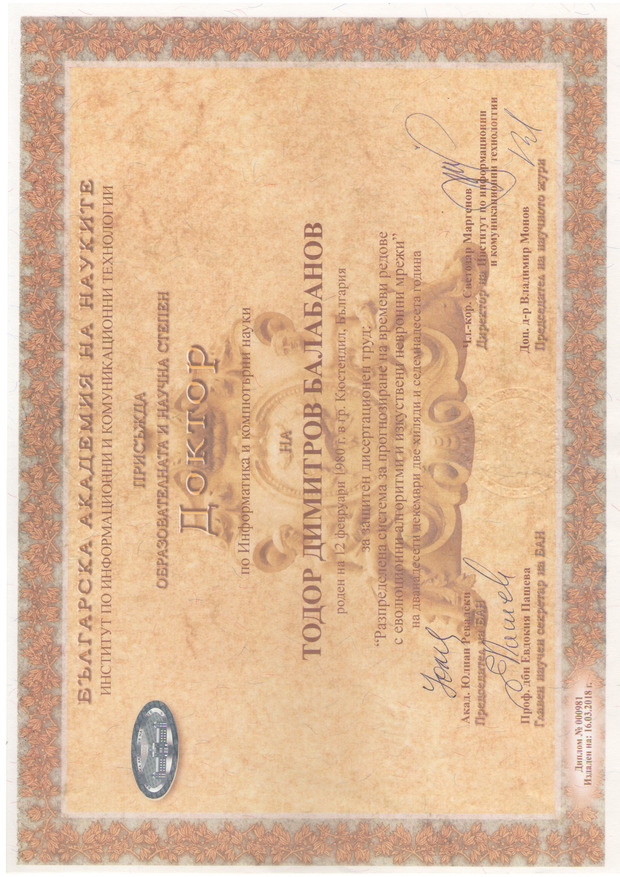
\includegraphics[width=\textwidth,height=\textheight,keepaspectratio]{DiplomaIICT2018}
%
%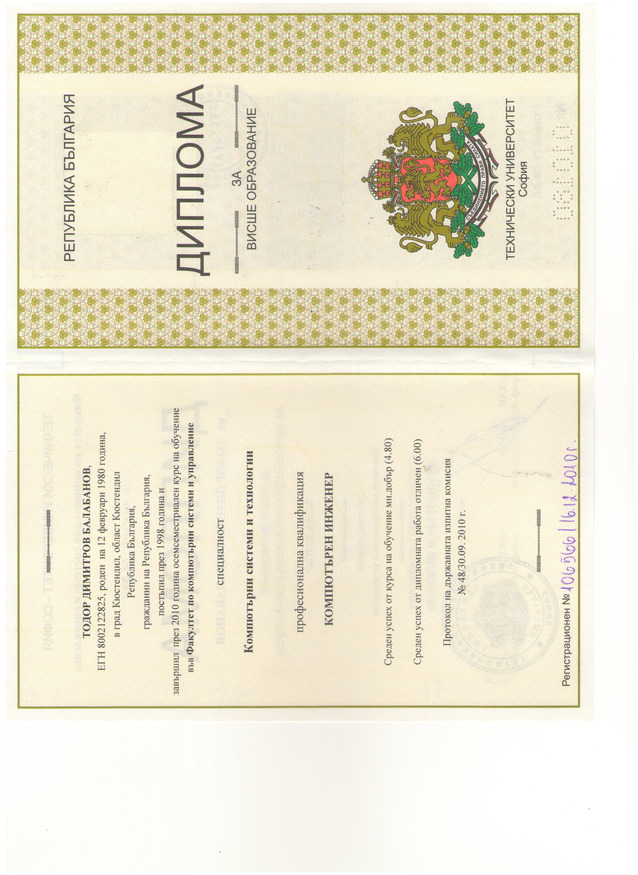
\includegraphics[width=\textwidth,height=\textheight,keepaspectratio]{DiplomaTU2010_1}
%
%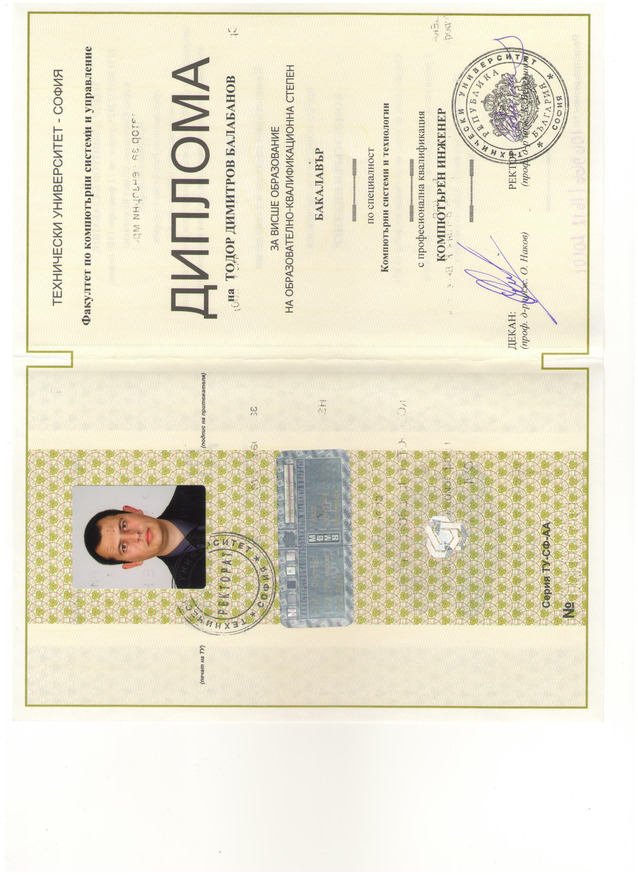
\includegraphics[width=\textwidth,height=\textheight,keepaspectratio]{DiplomaTU2010_2}
%
%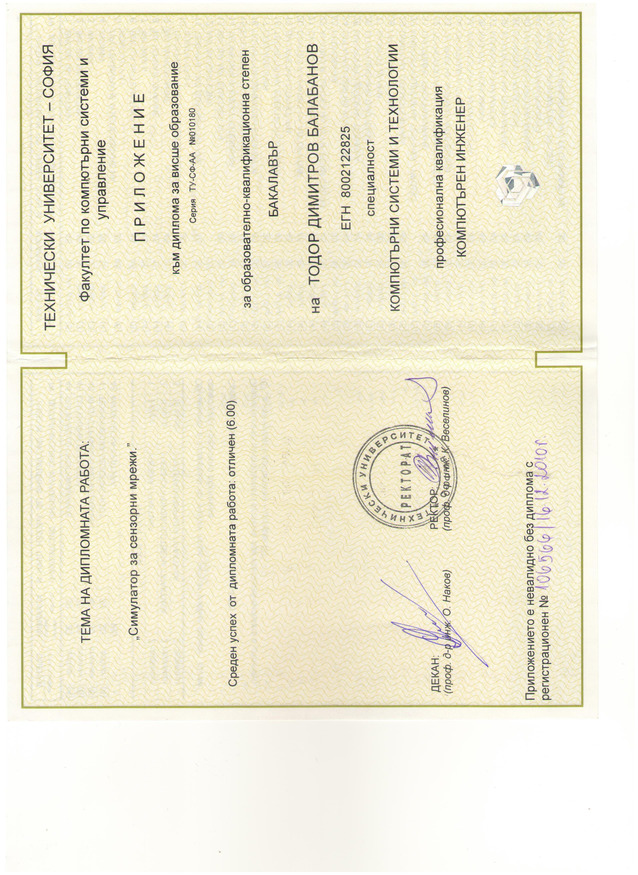
\includegraphics[width=\textwidth,height=\textheight,keepaspectratio]{DiplomaTU2010_3}
%
%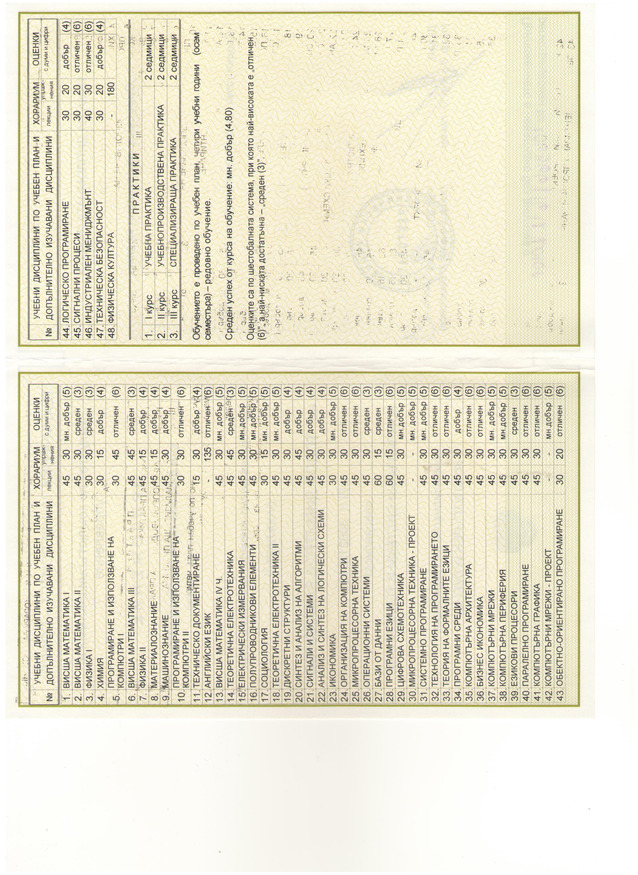
\includegraphics[width=\textwidth,height=\textheight,keepaspectratio]{DiplomaTU2010_4}
%
%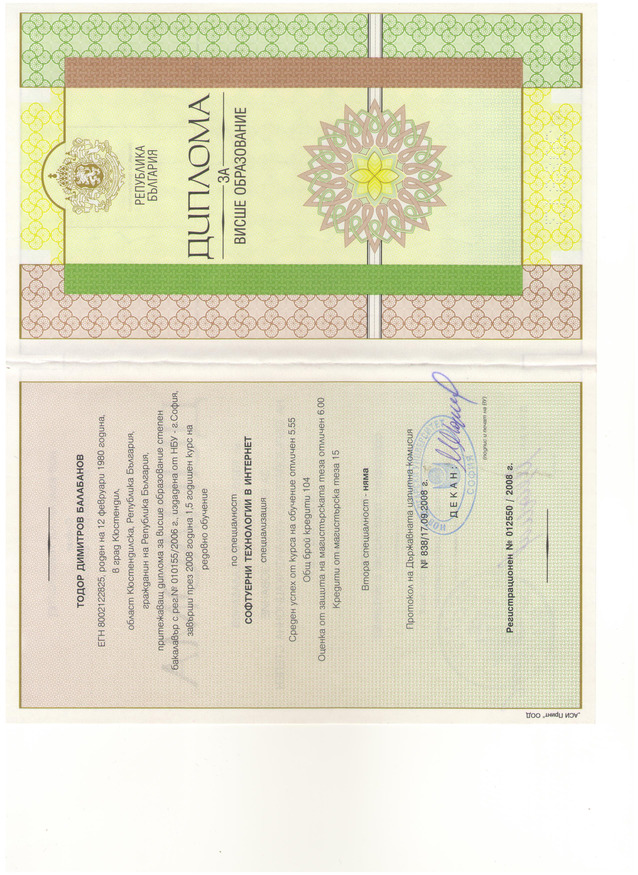
\includegraphics[width=\textwidth,height=\textheight,keepaspectratio]{DiplomaNBU2008_1}
%
%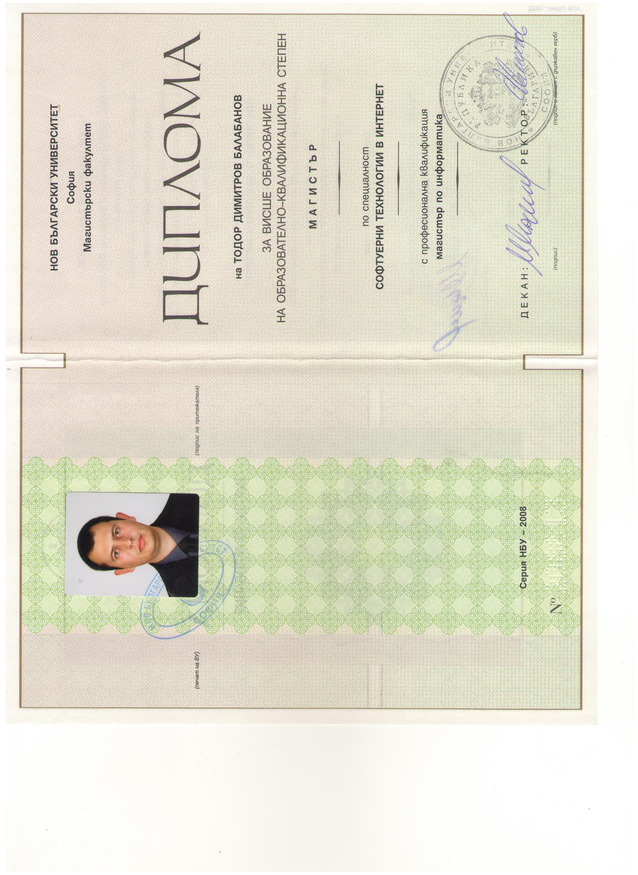
\includegraphics[width=\textwidth,height=\textheight,keepaspectratio]{DiplomaNBU2008_2}
%
%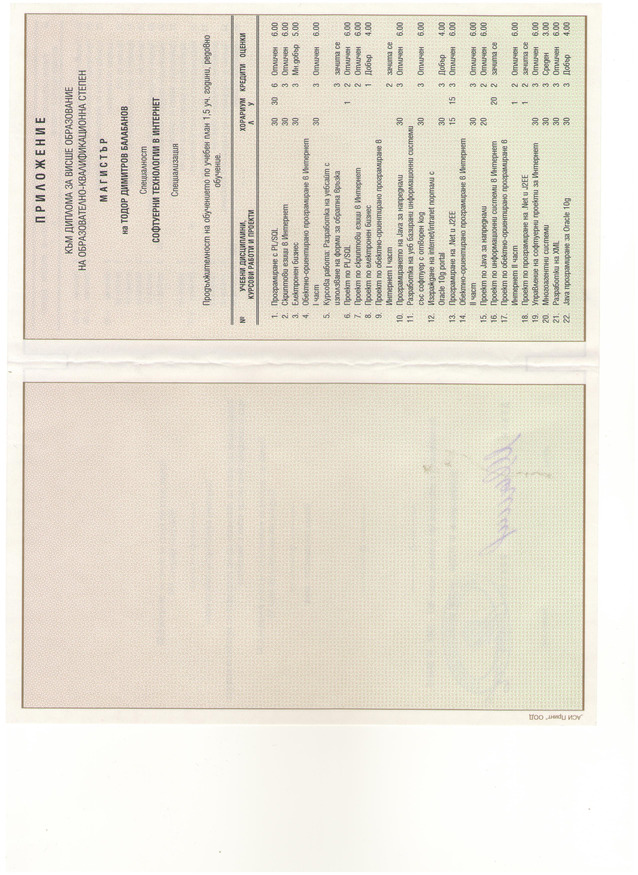
\includegraphics[width=\textwidth,height=\textheight,keepaspectratio]{DiplomaNBU2008_3}
%
%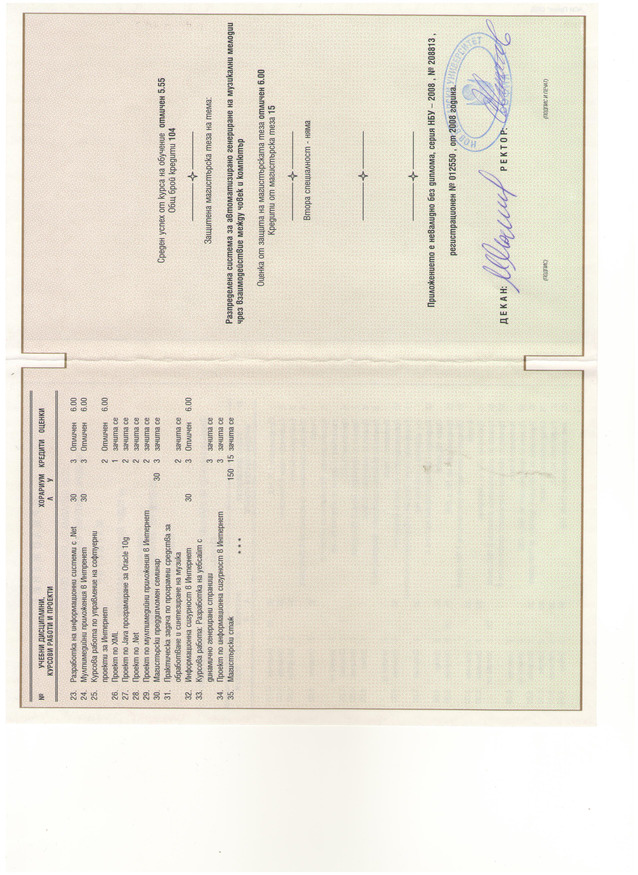
\includegraphics[width=\textwidth,height=\textheight,keepaspectratio]{DiplomaNBU2008_4}
%
%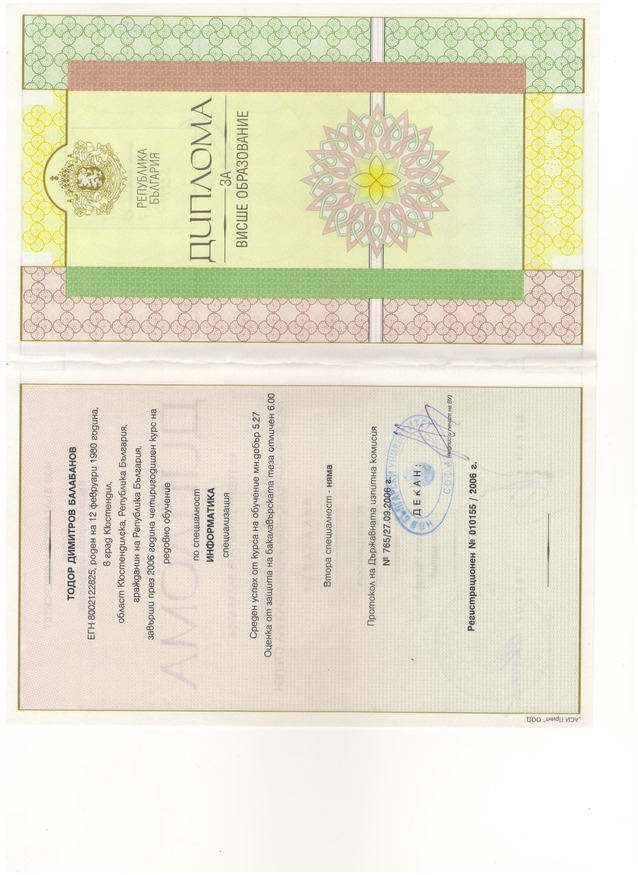
\includegraphics[width=\textwidth,height=\textheight,keepaspectratio]{DiplomaNBU2006_1}
%
%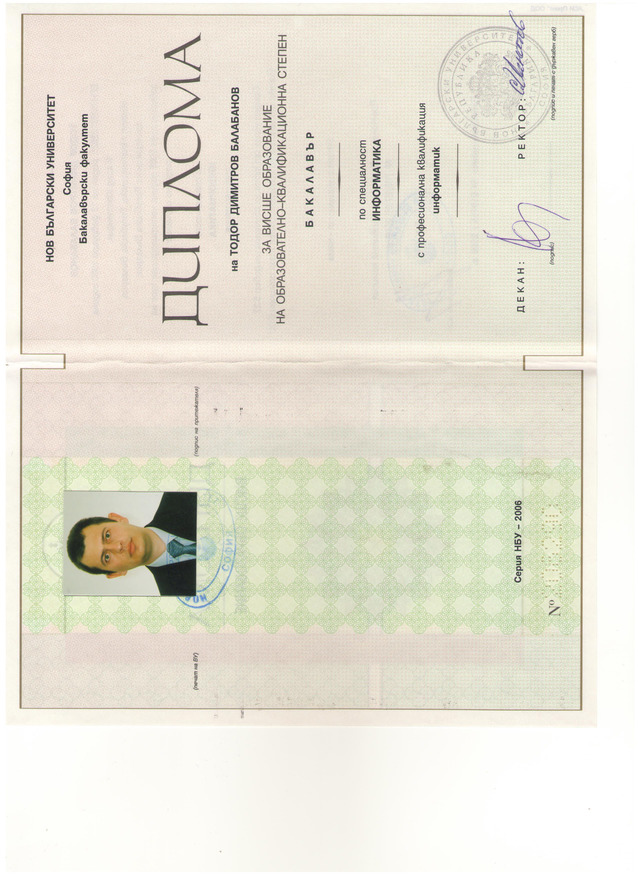
\includegraphics[width=\textwidth,height=\textheight,keepaspectratio]{DiplomaNBU2006_2}
%
%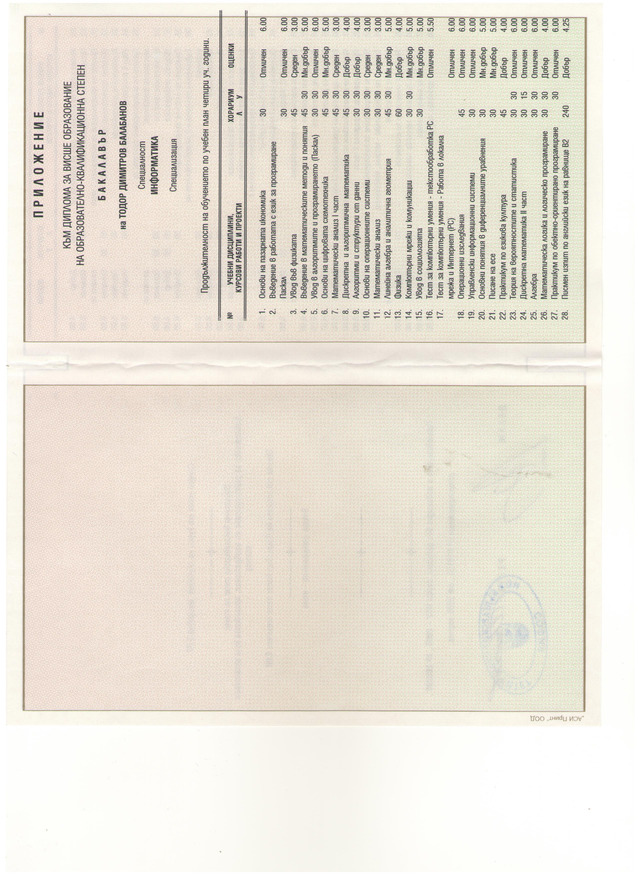
\includegraphics[width=\textwidth,height=\textheight,keepaspectratio]{DiplomaNBU2006_3}
%
%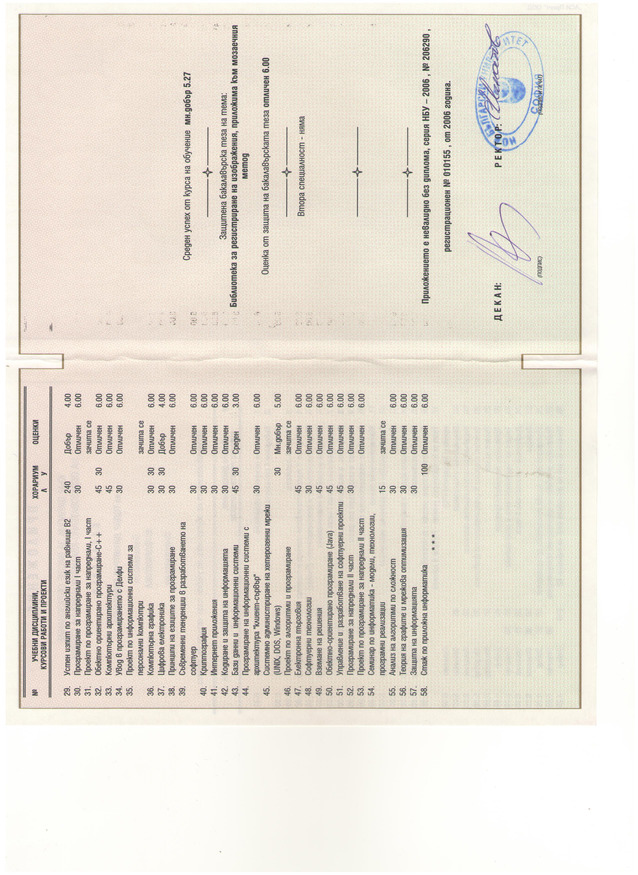
\includegraphics[width=\textwidth,height=\textheight,keepaspectratio]{DiplomaNBU2006_4}
%
%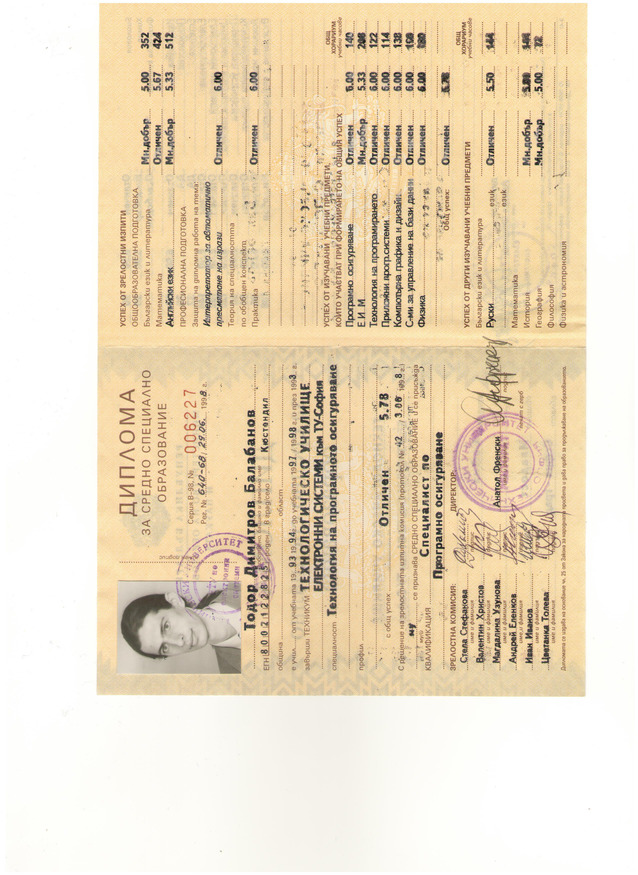
\includegraphics[width=\textwidth,height=\textheight,keepaspectratio]{DiplomaTUES1998_1}
%
%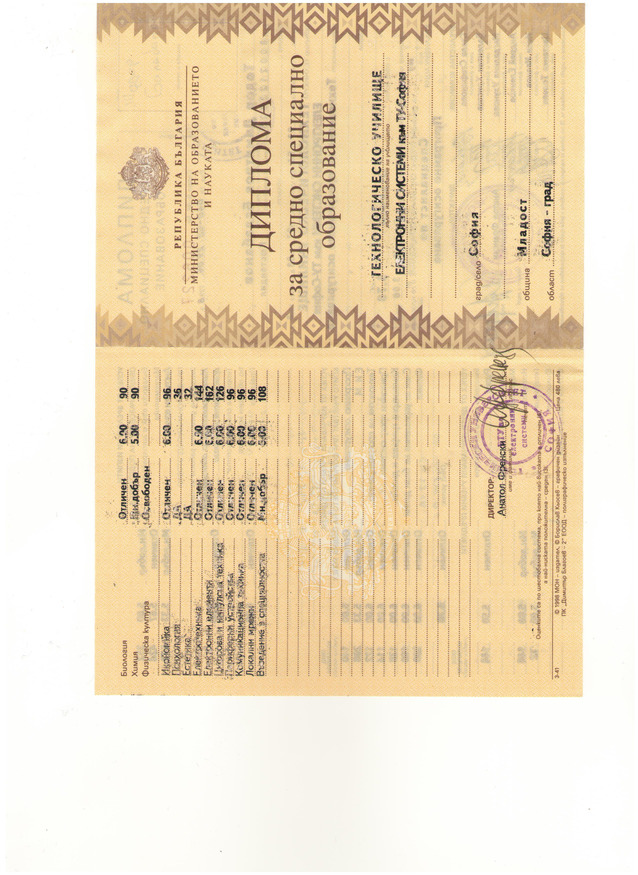
\includegraphics[width=\textwidth,height=\textheight,keepaspectratio]{DiplomaTUES1998_2}
%
%%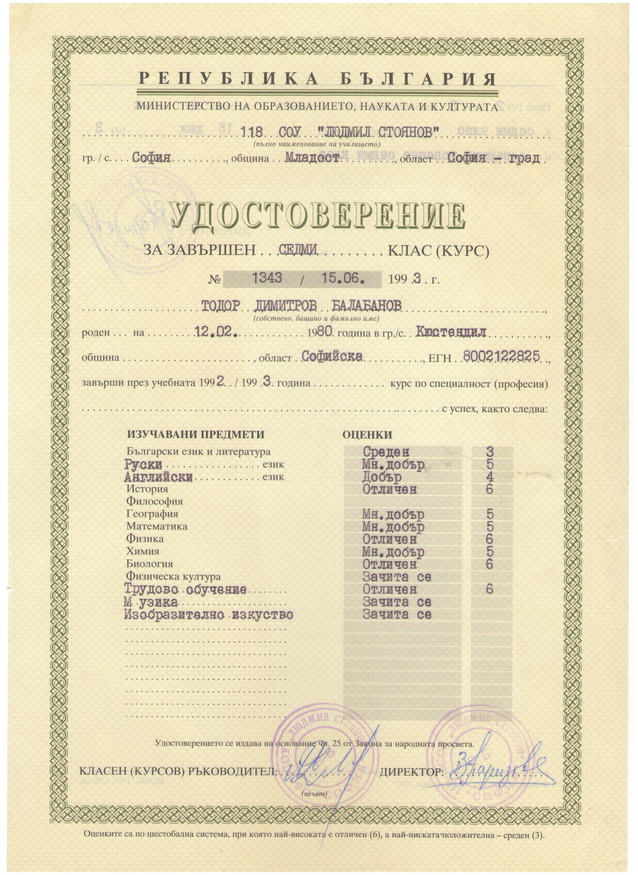
\includegraphics[width=\textwidth,height=\textheight,keepaspectratio]{118SOU1993_1}
%
%%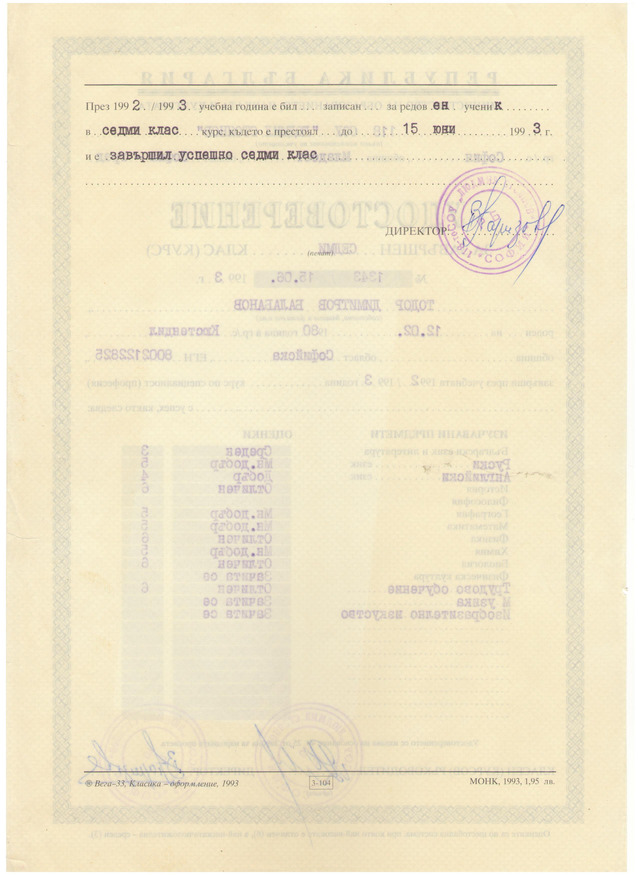
\includegraphics[width=\textwidth,height=\textheight,keepaspectratio]{118SOU1993_2}
%
%%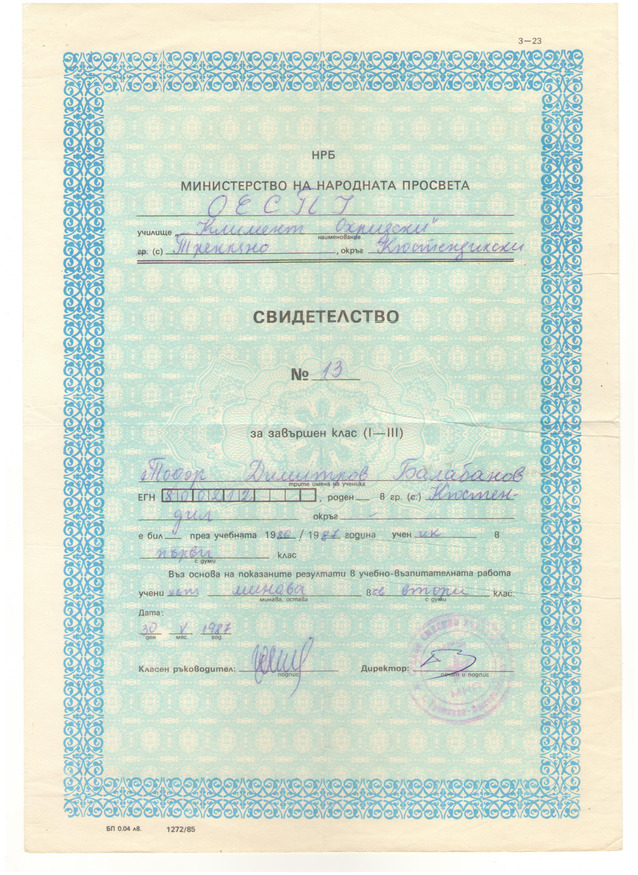
\includegraphics[width=\textwidth,height=\textheight,keepaspectratio]{OESPU1987}
%
%
\includegraphics[width=\textwidth,height=\textheight,keepaspectratio]{Karoll2019}
%
%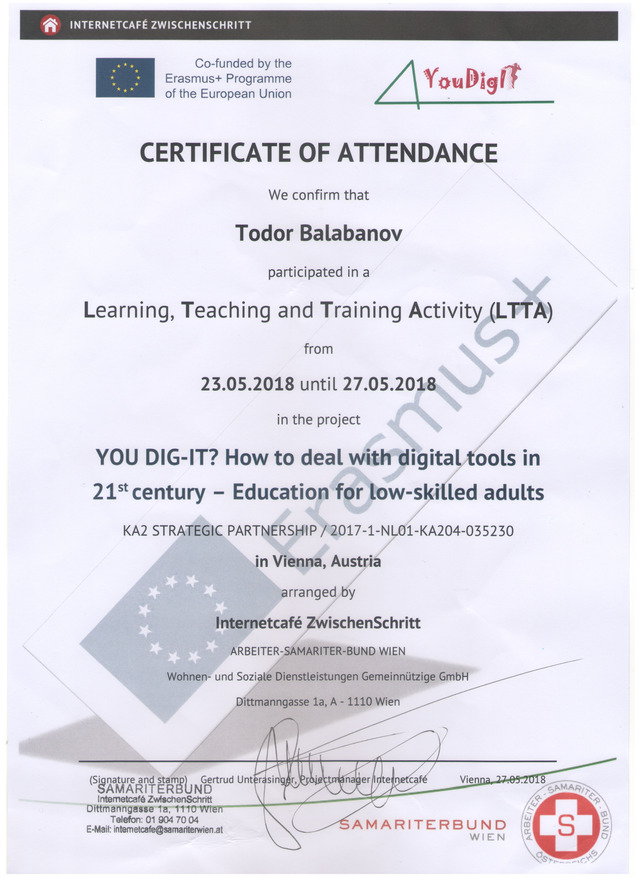
\includegraphics[width=\textwidth,height=\textheight,keepaspectratio]{YouDigIT2018}
%
%
\includegraphics[width=\textwidth,height=\textheight,keepaspectratio]{ESGI1322017}
%
%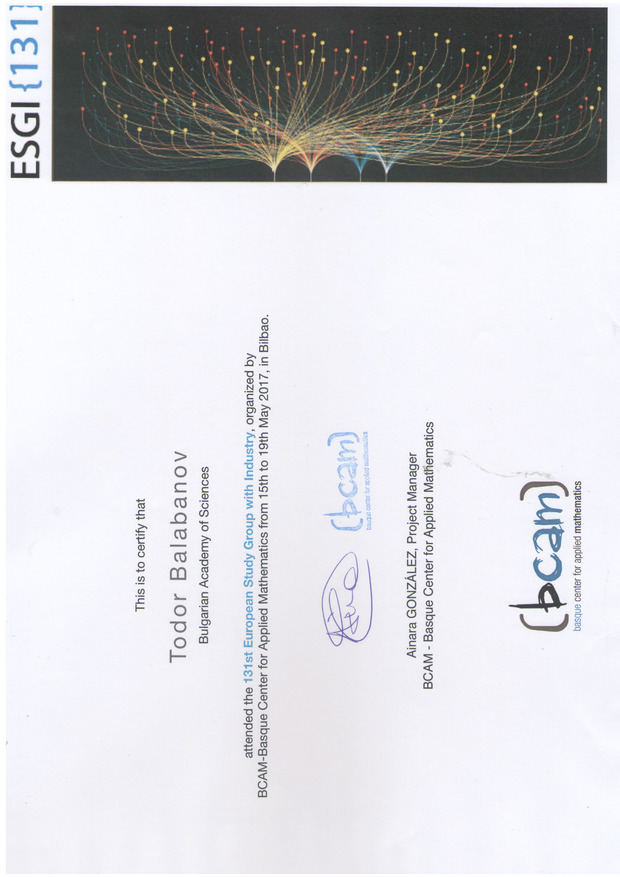
\includegraphics[width=\textwidth,height=\textheight,keepaspectratio]{131ESGI2017}
%
%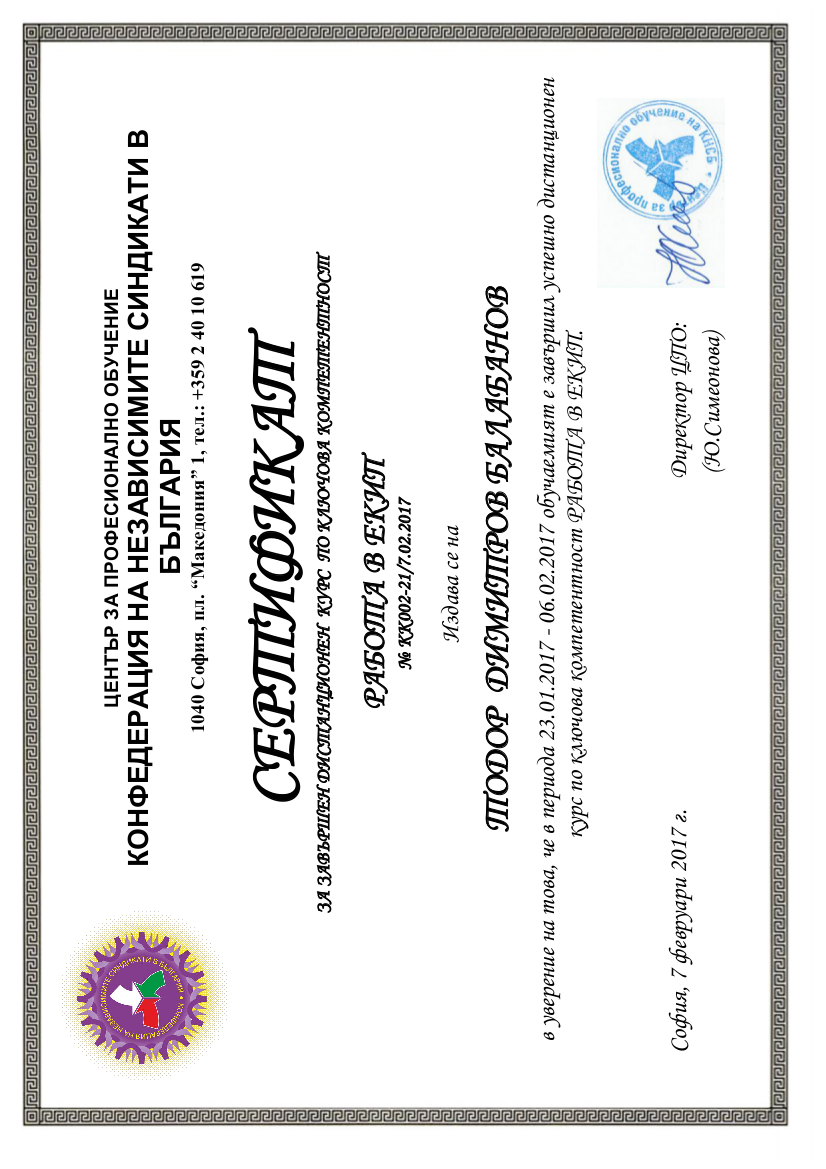
\includegraphics[width=\textwidth,height=\textheight,keepaspectratio]{KNSB2017_1}
%
%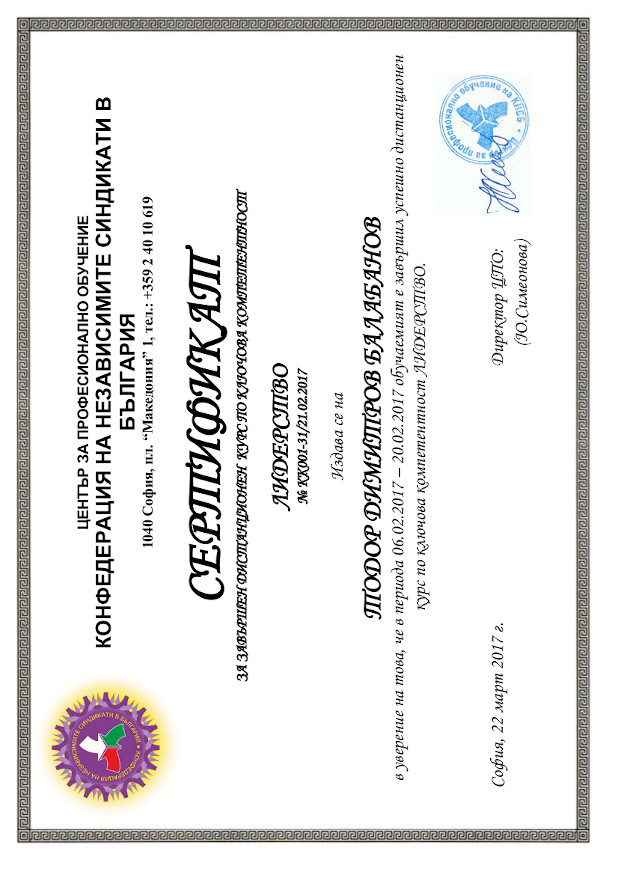
\includegraphics[width=\textwidth,height=\textheight,keepaspectratio]{KNSB2017_2}
%
%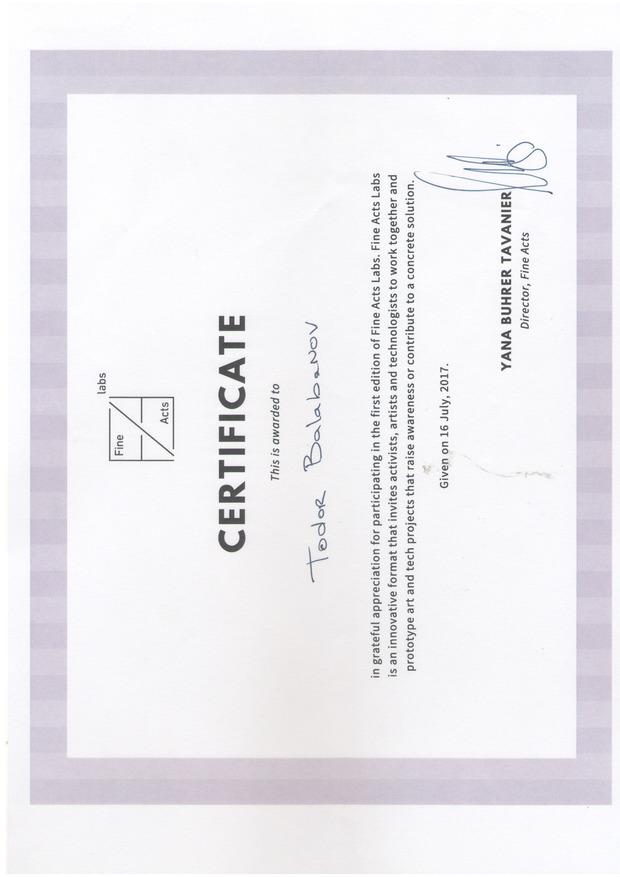
\includegraphics[width=\textwidth,height=\textheight,keepaspectratio]{FineActsLabs2017}
%
%
\includegraphics[width=\textwidth,height=\textheight,keepaspectratio]{InfoTech2016}
%
%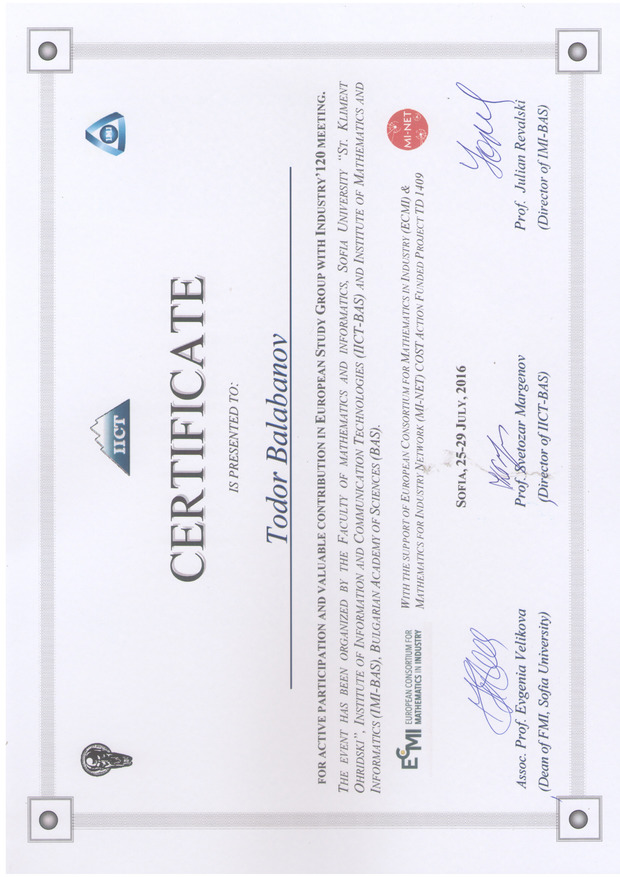
\includegraphics[width=\textwidth,height=\textheight,keepaspectratio]{ESGI1202016}
%
%
\includegraphics[width=\textwidth,height=\textheight,keepaspectratio]{MA2016}
%
%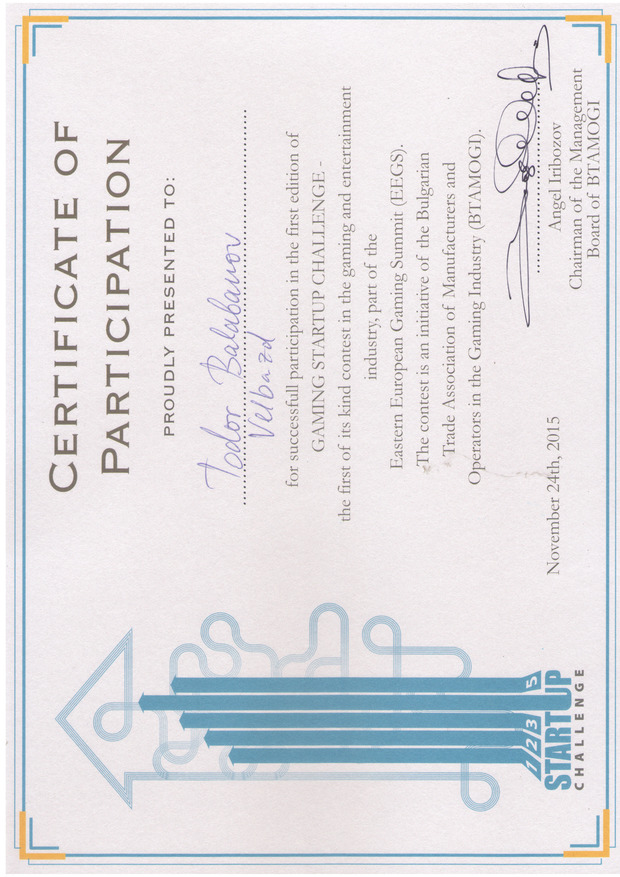
\includegraphics[width=\textwidth,height=\textheight,keepaspectratio]{EEGS2015}
%
%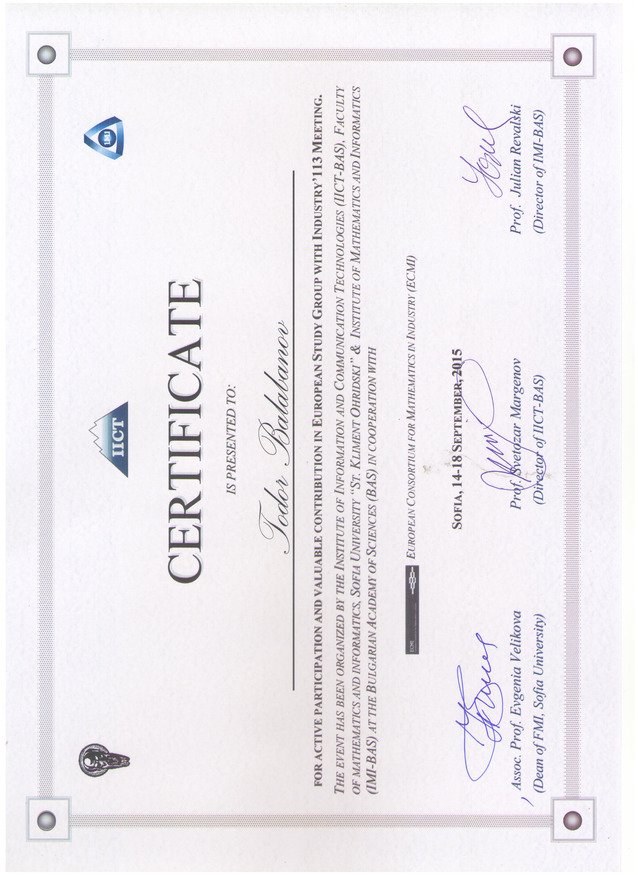
\includegraphics[width=\textwidth,height=\textheight,keepaspectratio]{ESGI1132015}
%
%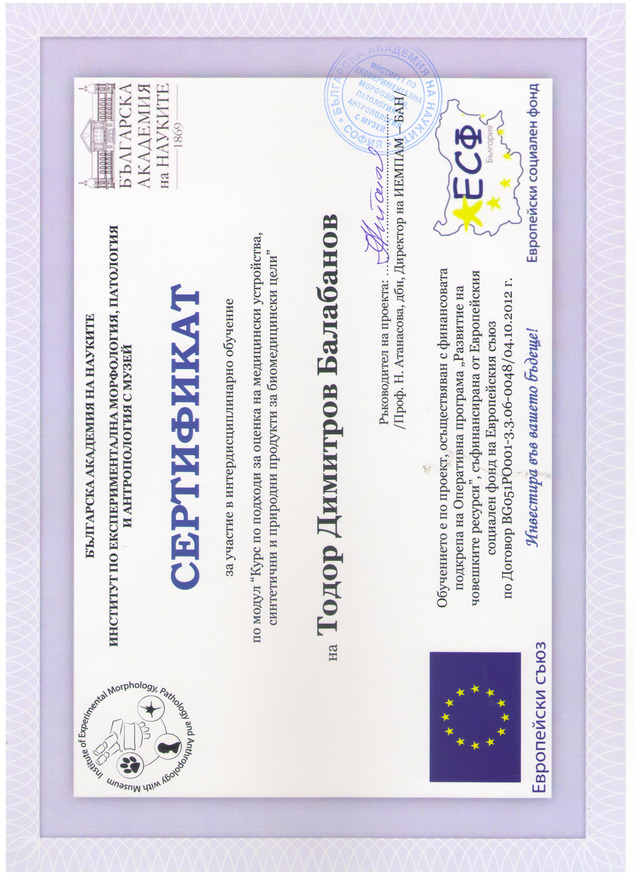
\includegraphics[width=\textwidth,height=\textheight,keepaspectratio]{IEMPAM2014_1}
%
%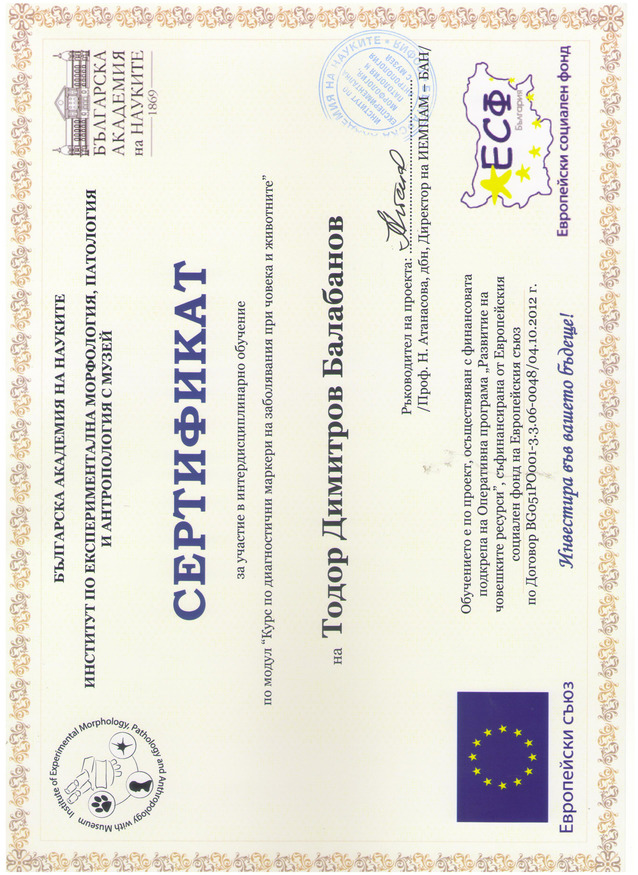
\includegraphics[width=\textwidth,height=\textheight,keepaspectratio]{IEMPAM2014_2}
%
%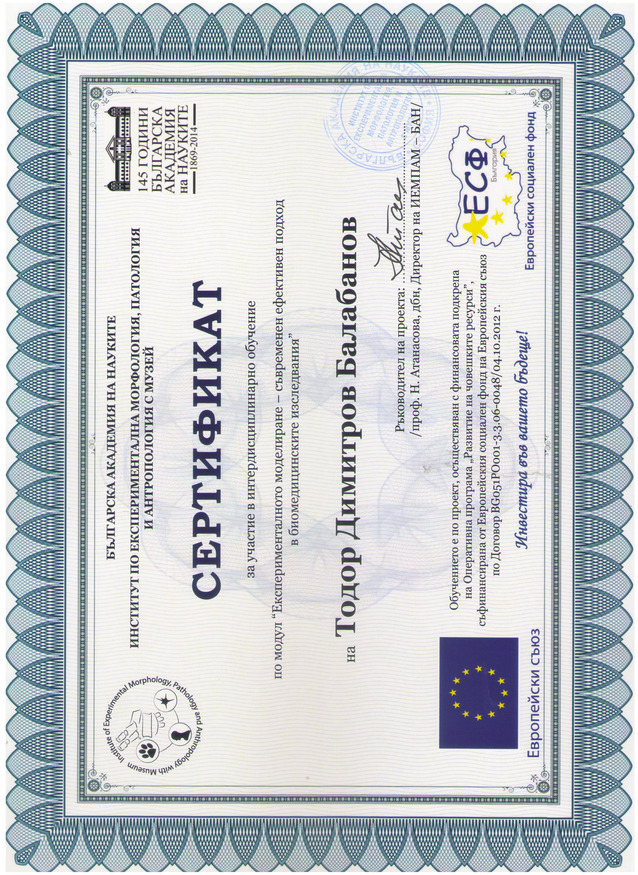
\includegraphics[width=\textwidth,height=\textheight,keepaspectratio]{IEMPAM2014_3}
%
%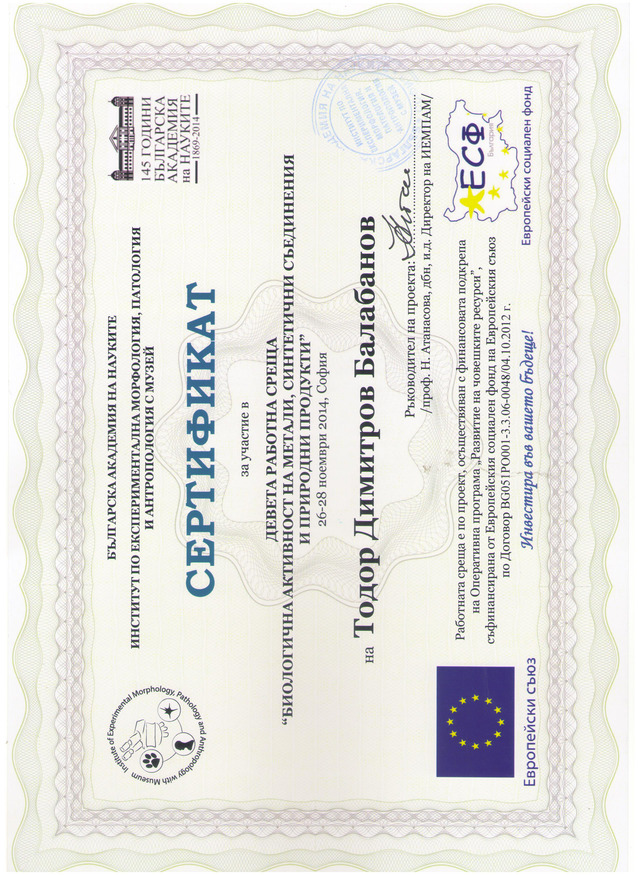
\includegraphics[width=\textwidth,height=\textheight,keepaspectratio]{IEMPAM2014_4}
%
%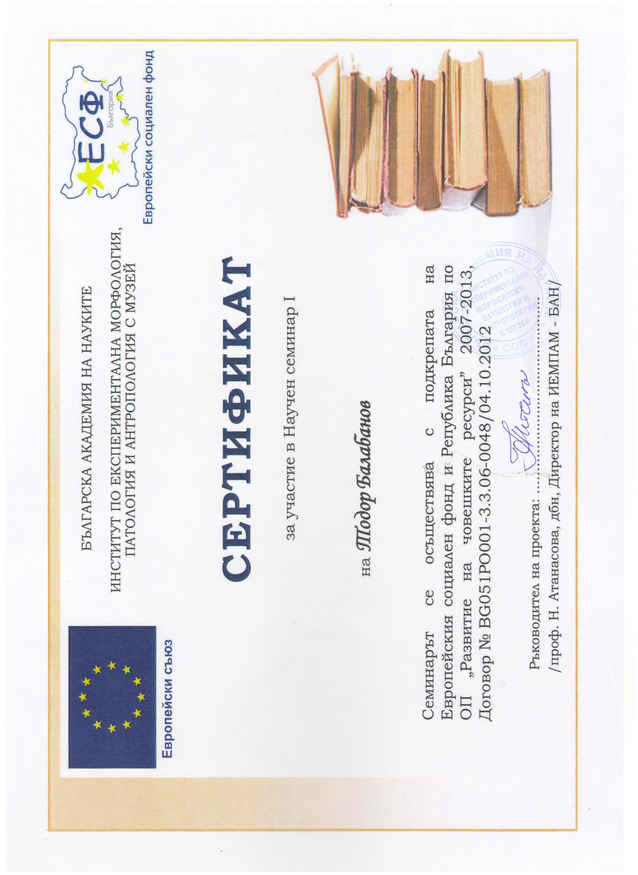
\includegraphics[width=\textwidth,height=\textheight,keepaspectratio]{IEMPAM2013_1}
%
%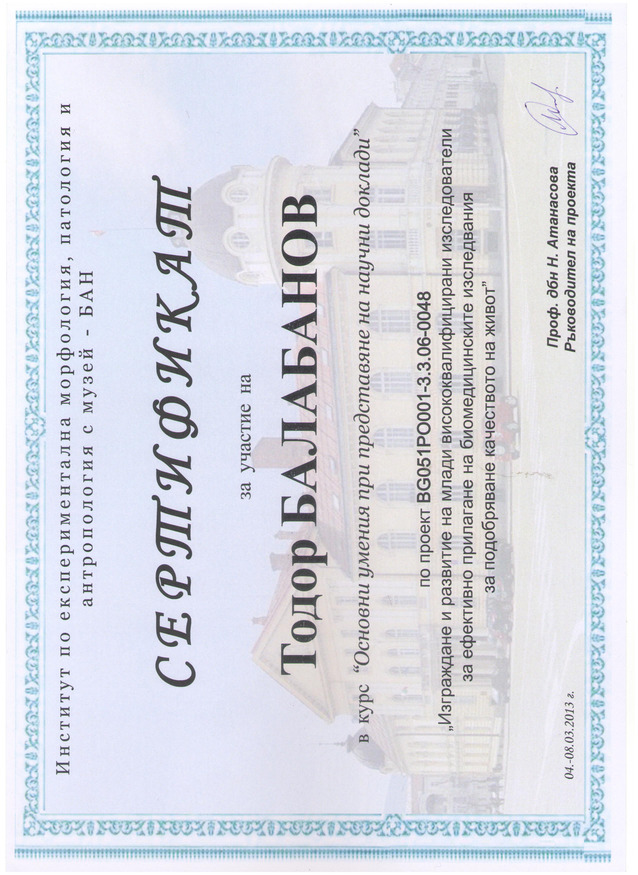
\includegraphics[width=\textwidth,height=\textheight,keepaspectratio]{IEMPAM2013_2}
%
%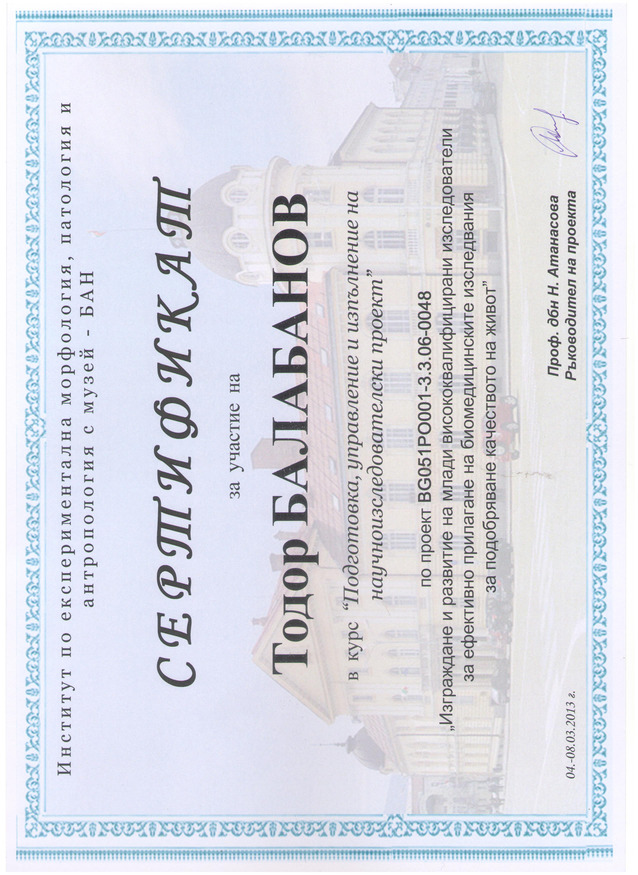
\includegraphics[width=\textwidth,height=\textheight,keepaspectratio]{IEMPAM2013_3}
%
%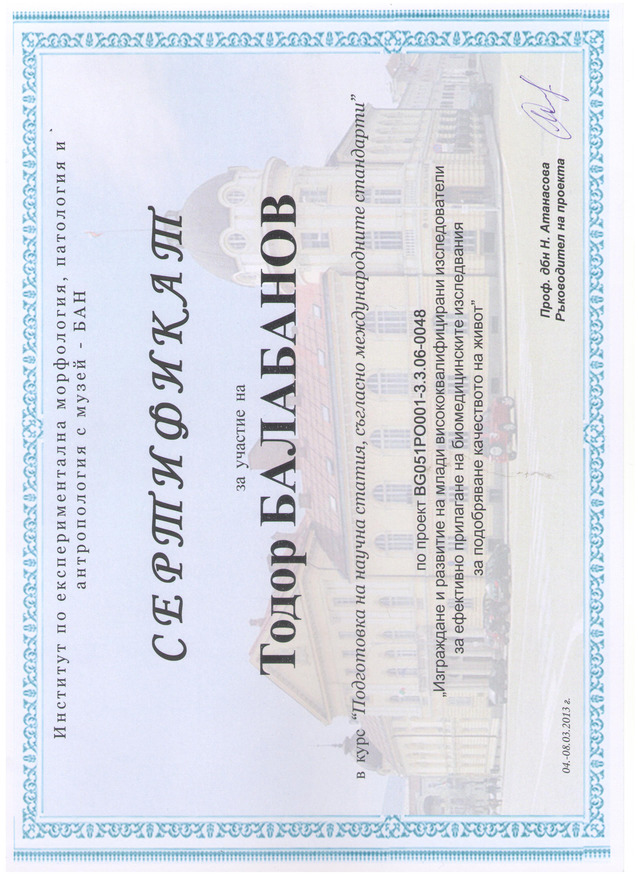
\includegraphics[width=\textwidth,height=\textheight,keepaspectratio]{IEMPAM2013_4}
%
%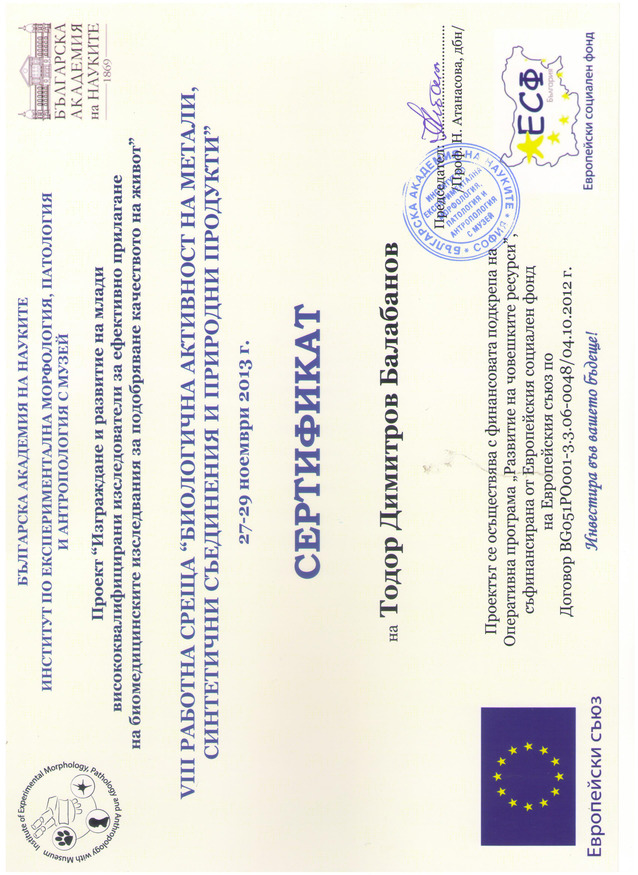
\includegraphics[width=\textwidth,height=\textheight,keepaspectratio]{IEMPAM2013_5}
%
%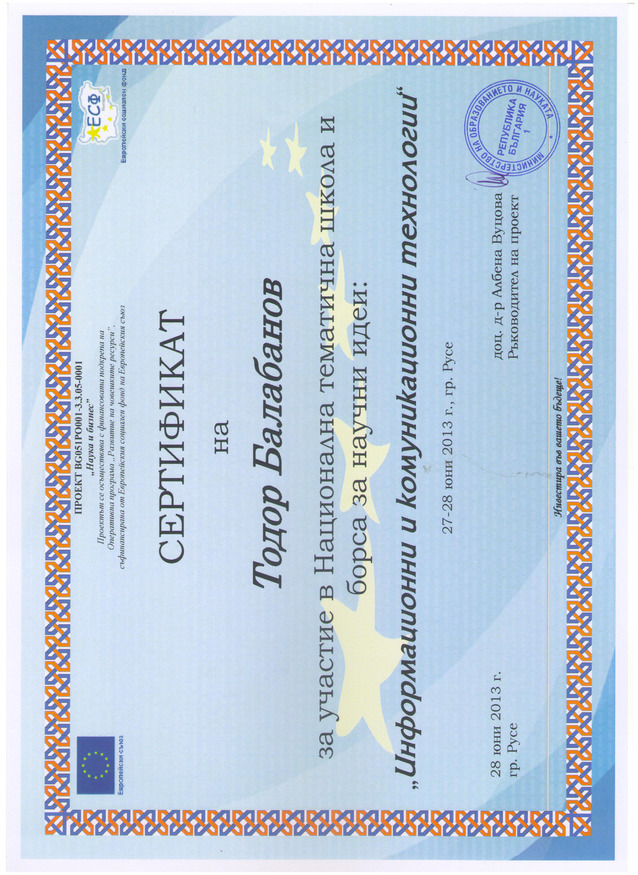
\includegraphics[width=\textwidth,height=\textheight,keepaspectratio]{Rouse2013}
%
%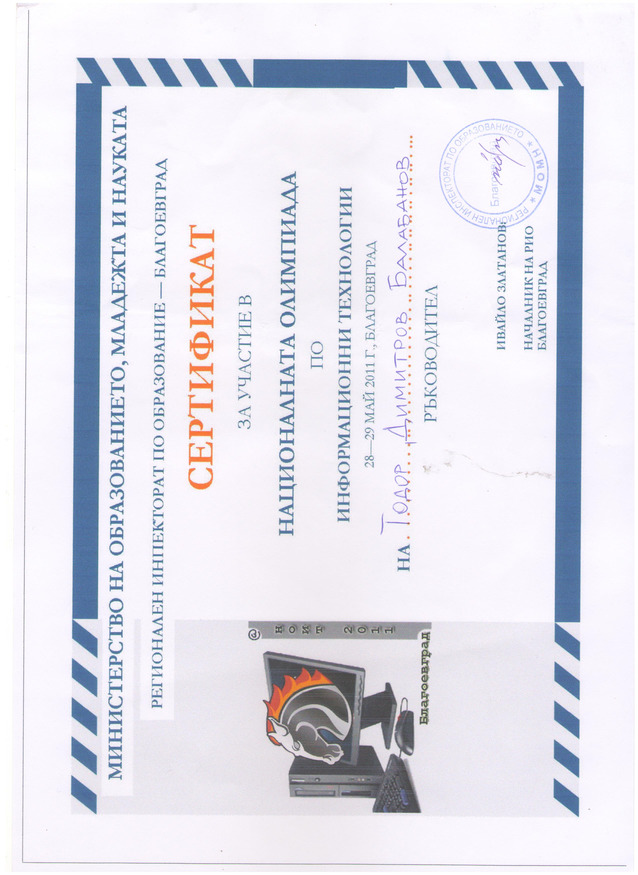
\includegraphics[width=\textwidth,height=\textheight,keepaspectratio]{ElSys2011}
%
%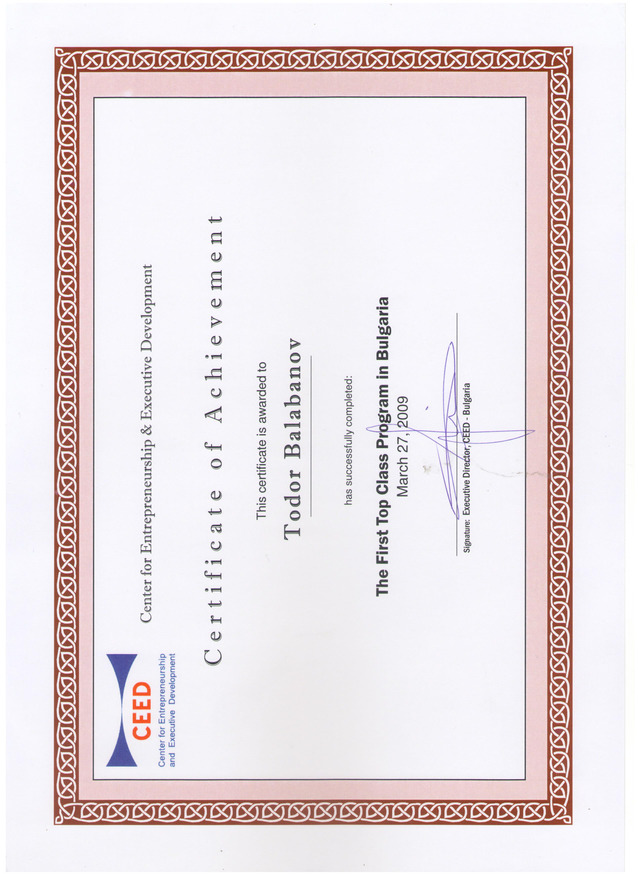
\includegraphics[width=\textwidth,height=\textheight,keepaspectratio]{CEED2009}
%
%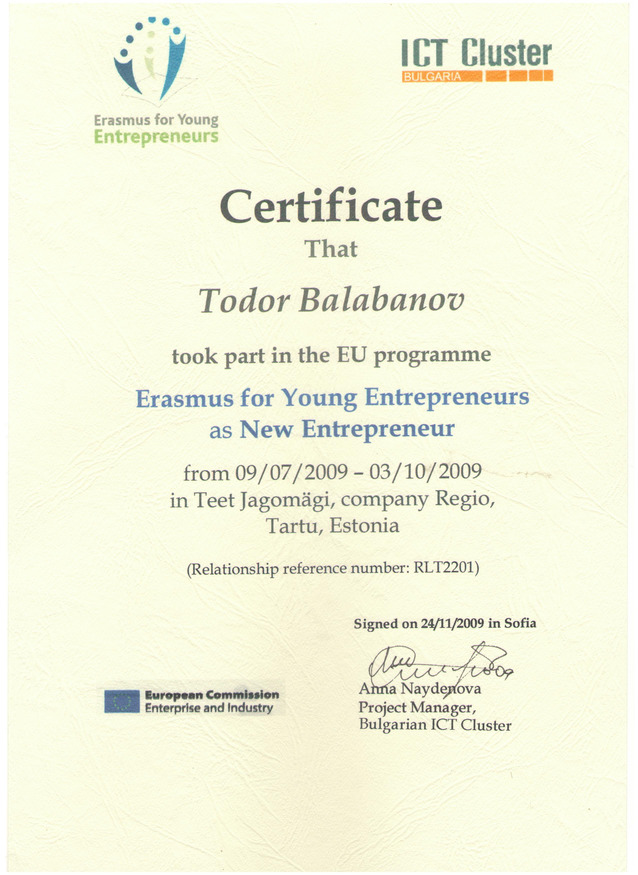
\includegraphics[width=\textwidth,height=\textheight,keepaspectratio]{EYE2009}
%
%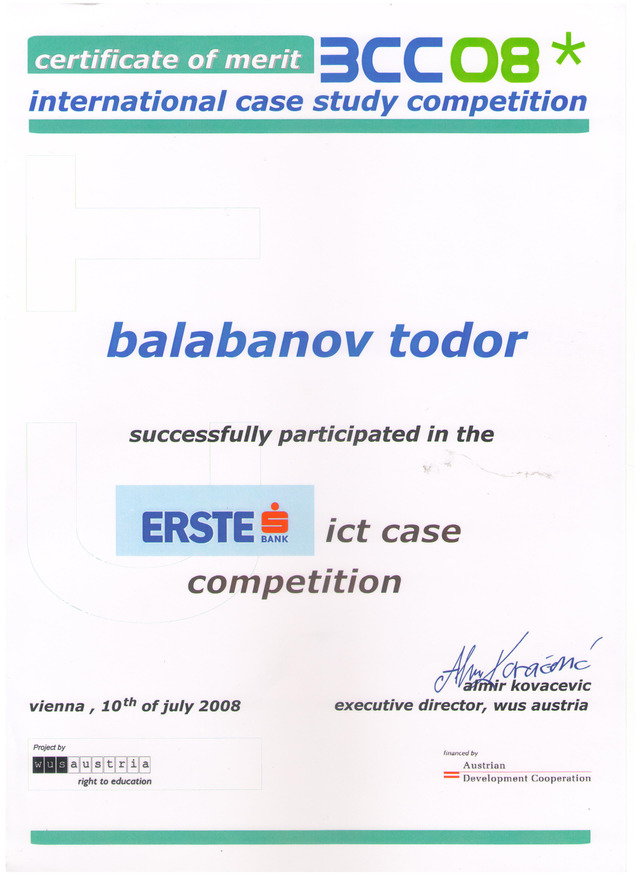
\includegraphics[width=\textwidth,height=\textheight,keepaspectratio]{BCC2008}
%
%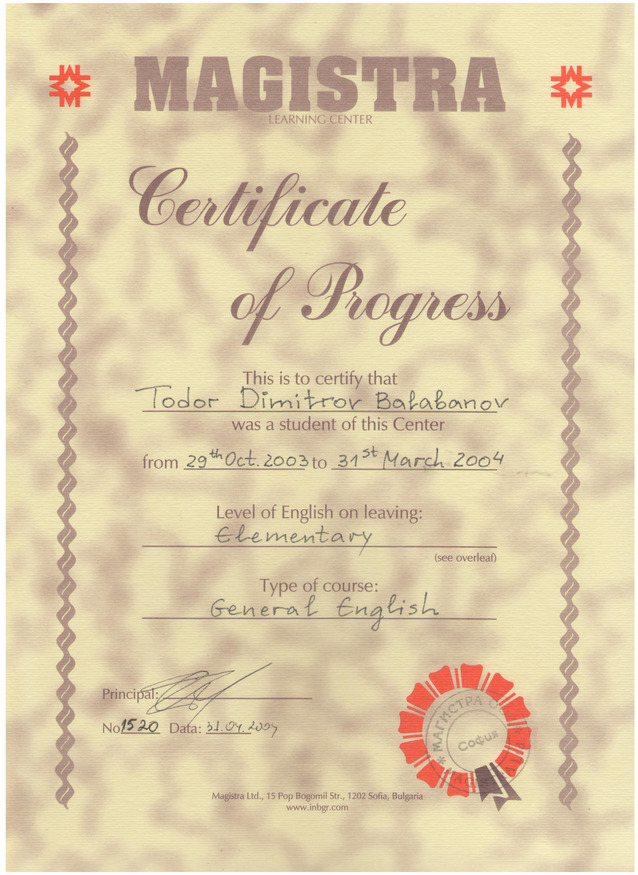
\includegraphics[width=\textwidth,height=\textheight,keepaspectratio]{Magistra2004}
%
%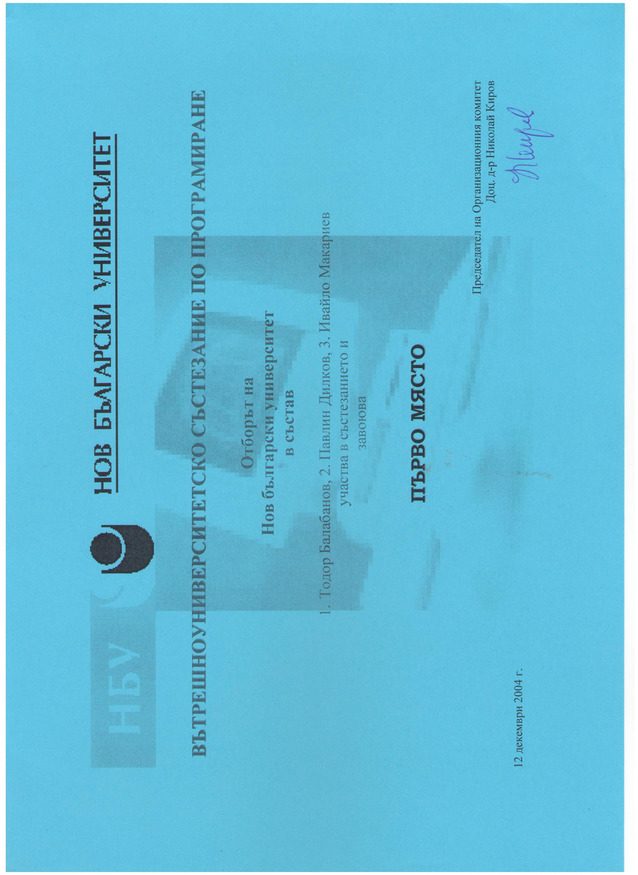
\includegraphics[width=\textwidth,height=\textheight,keepaspectratio]{NBU2004}
%
%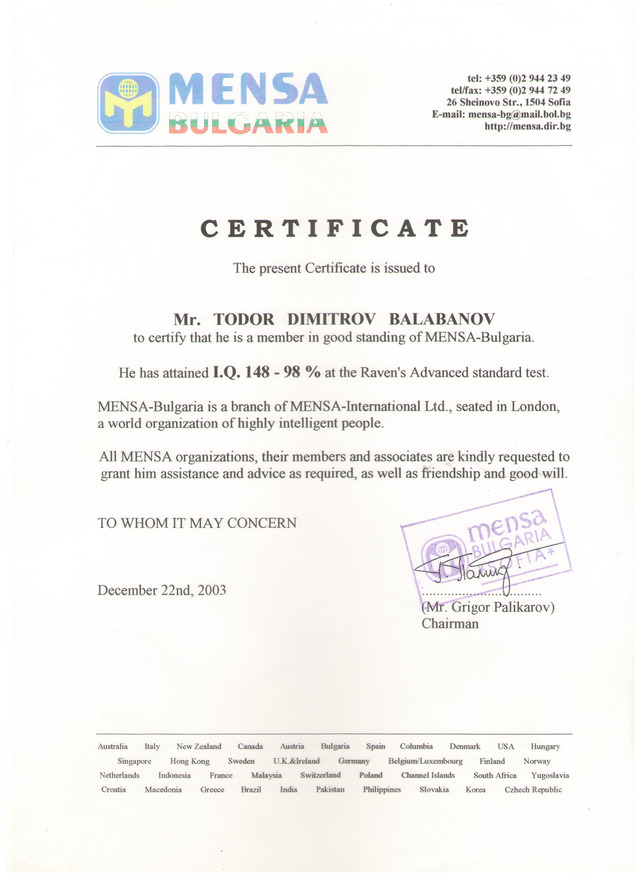
\includegraphics[width=\textwidth,height=\textheight,keepaspectratio]{Mensa2003}
%
%%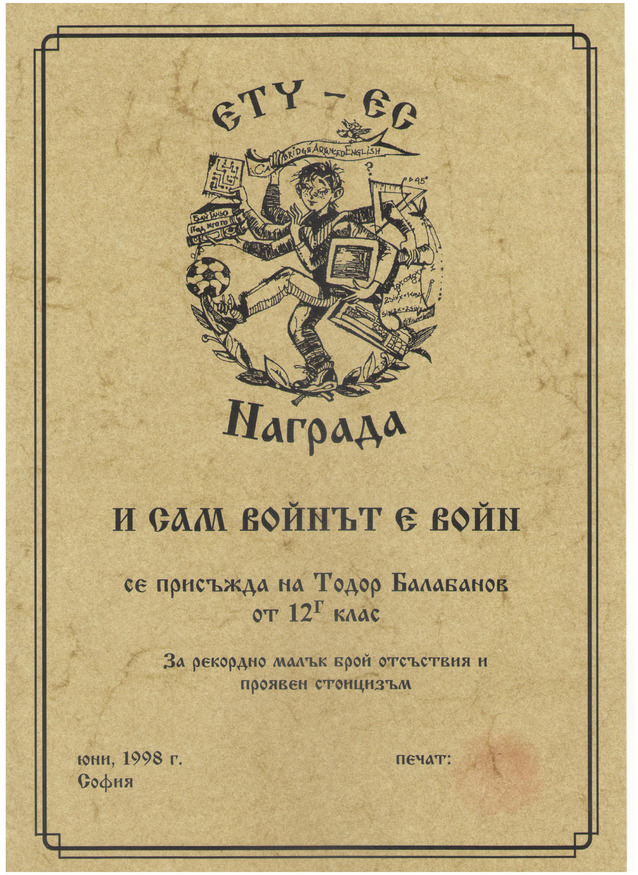
\includegraphics[width=\textwidth,height=\textheight,keepaspectratio]{ElSys1998}
%
%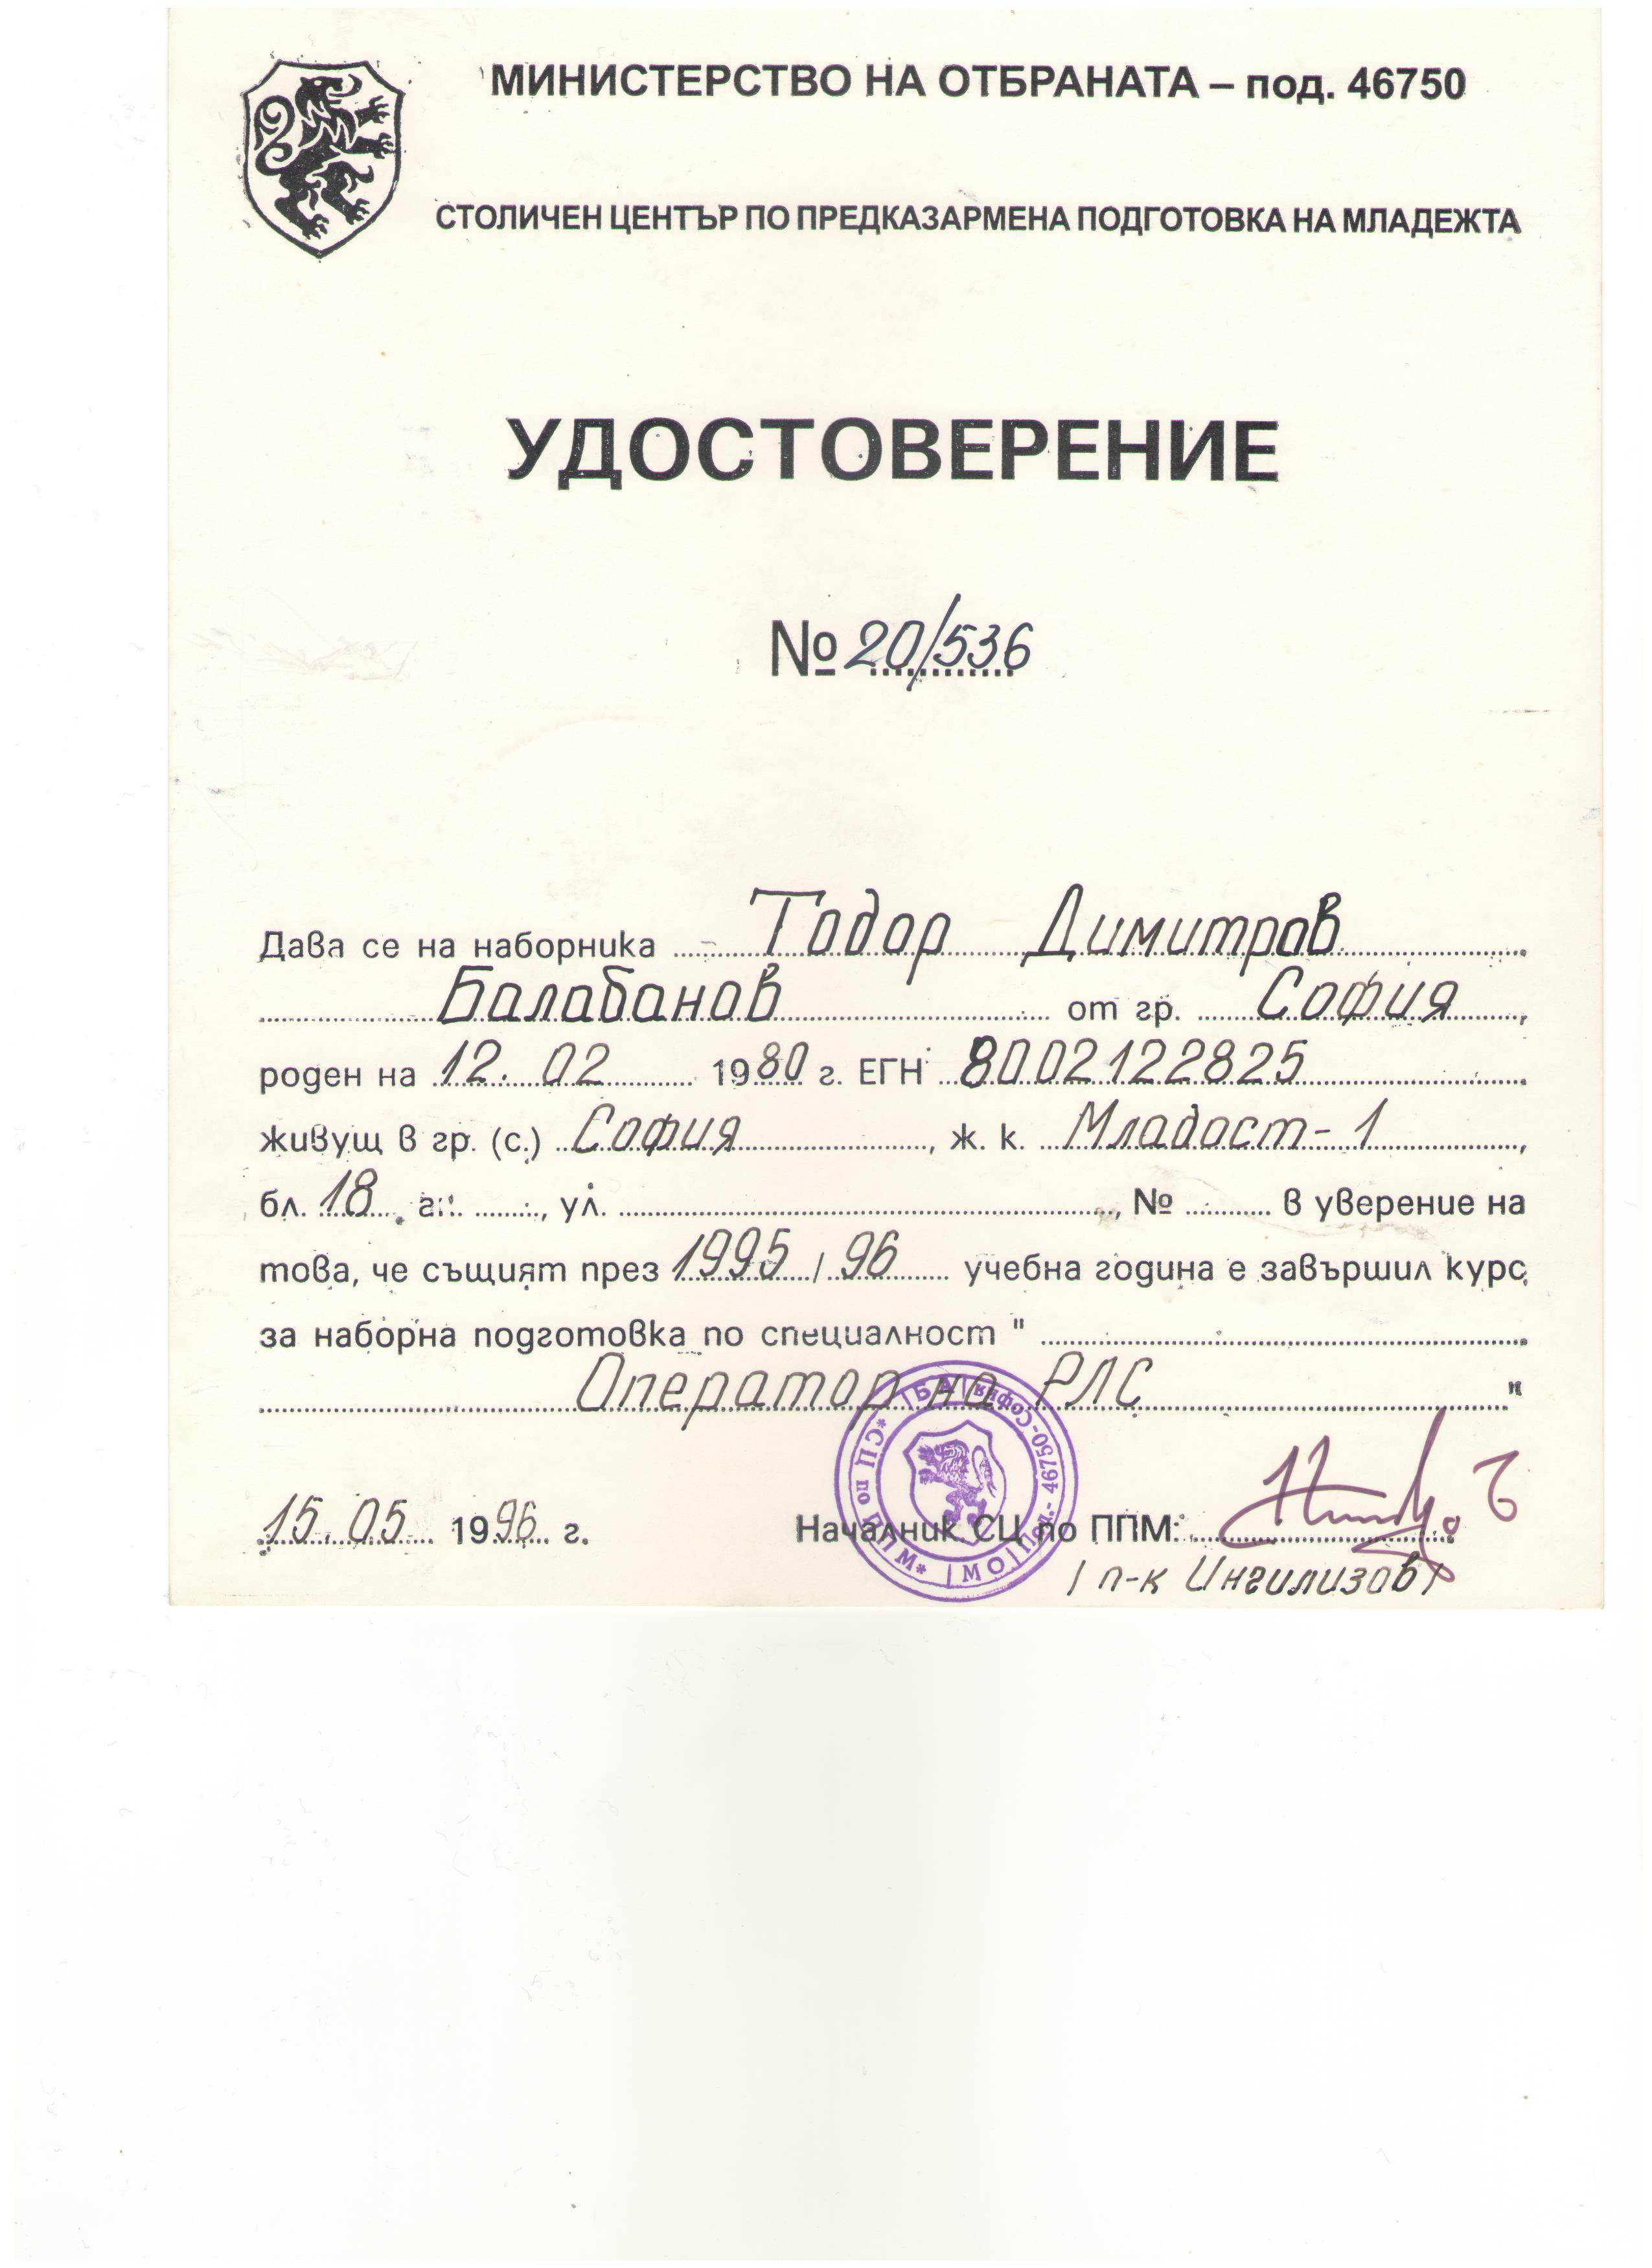
\includegraphics[width=\textwidth,height=\textheight,keepaspectratio]{MO1996}

\end{document}